%! Author = melek
%! Date = 22.01.2023

% Preamble
\documentclass[11pt]{article}

% Packages
\usepackage{amsmath}
\usepackage{graphicx}
\graphicspath{ {../images/} }

\title{Assignment 5: Exploration Strategies and Offline Reinforcement Learning}
\author{huseyinabanox@gmail.com}
\date{February 2023}

% Document
\begin{document}

    \maketitle

    Each experiment is run using 4 different seeds and their average is displayed.
    Training return is average of the last 100 training step rewards.
    Evaluation return is average of the 1000 evaluation step rewards.

    \section{Part 1: “Unsupervised” RND and exploration performance}

    \subsection{RND Implementation}

    Experiments are run using easy, medium and hard environments.
    Relevant notebooks with plots can be found and report package.

    \subsubsection{Easy Environment}

    Expectation 1: For debugging this problem, note that on the easy environment we would expect to obtain a mean reward (100 episodes) of -25 within 4000 iterations of online exploitation.

    Online exploitation starts after 10K iterations.
    Plus 4K iteration sums to 14K iteration.
    We are required to reach a mean reward of -25 within 14K iterations.

    \hspace*{-0.6in}
    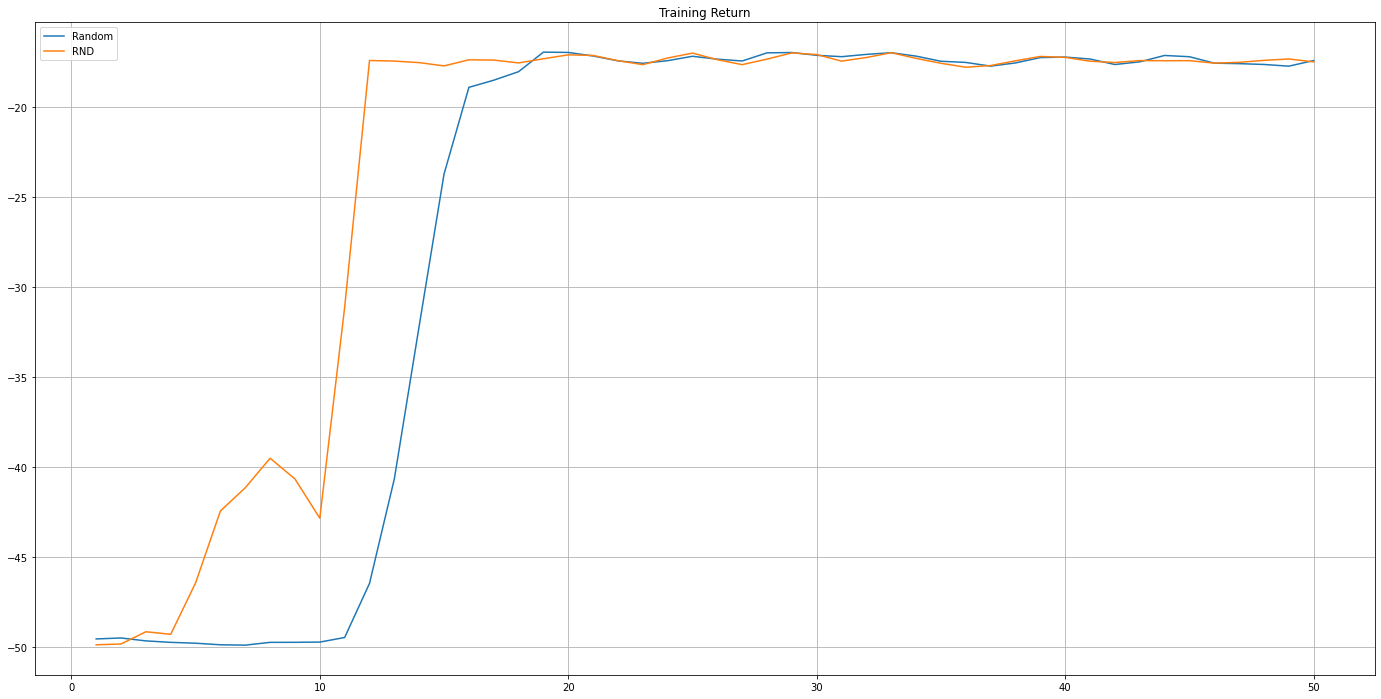
\includegraphics[scale=0.30]{q1/q1-easy-train-compare}

    The chart shows both exploration strategies reach the target mean reward within 14K iterations.
    The RND strategy reaches the target immediately after the beginning of the online exploitation.

    \hspace*{-0.6in}
    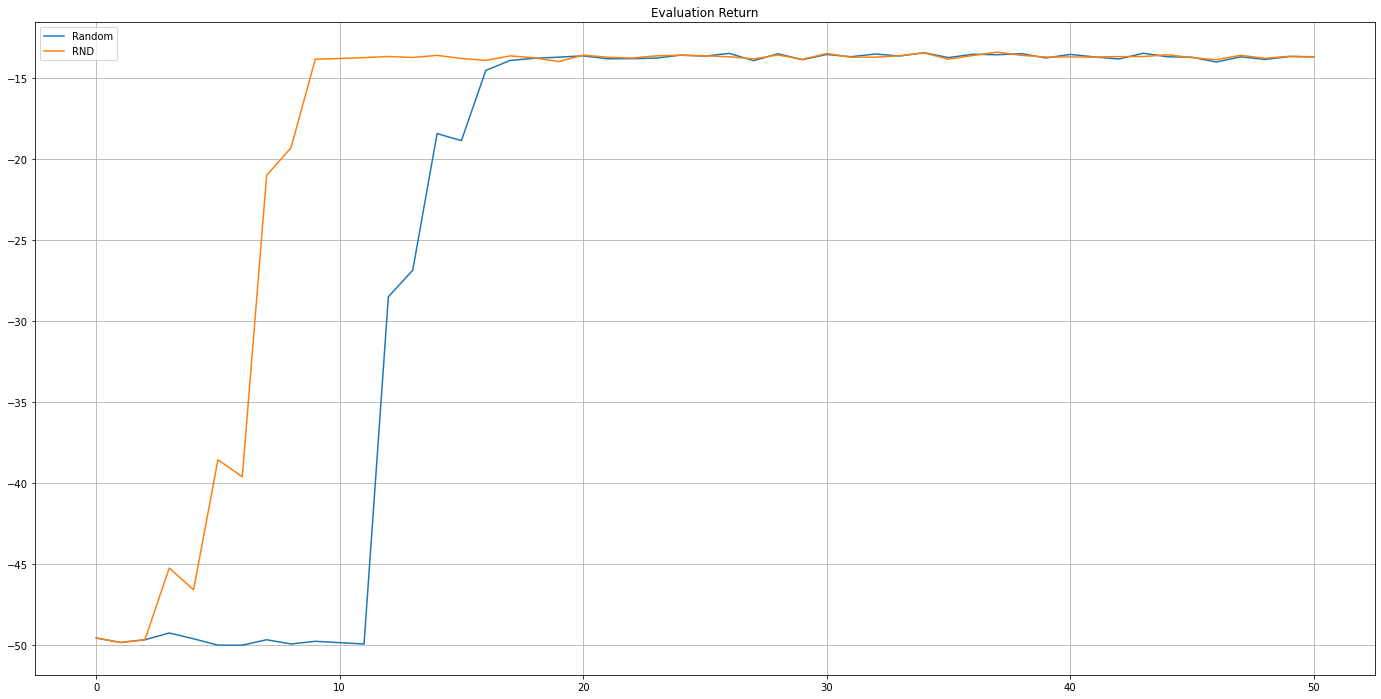
\includegraphics[scale=0.30]{q1/q1-easy-eval-compare}

    In terms of evaluation performance, both strategies perform the same.
    Note that random strategy starts learning after 10K steps while RND strategy starts learning after 2K steps.



    Expectation 2: The density of the state-action pairs on this easy environment is, as expected, more uniformly spread over the reachable parts of the environment (that are not occupied by walls) with RND as compared to random exploration where most of the density would be concentrated around the starting state.

    \hspace*{-0.6in}
    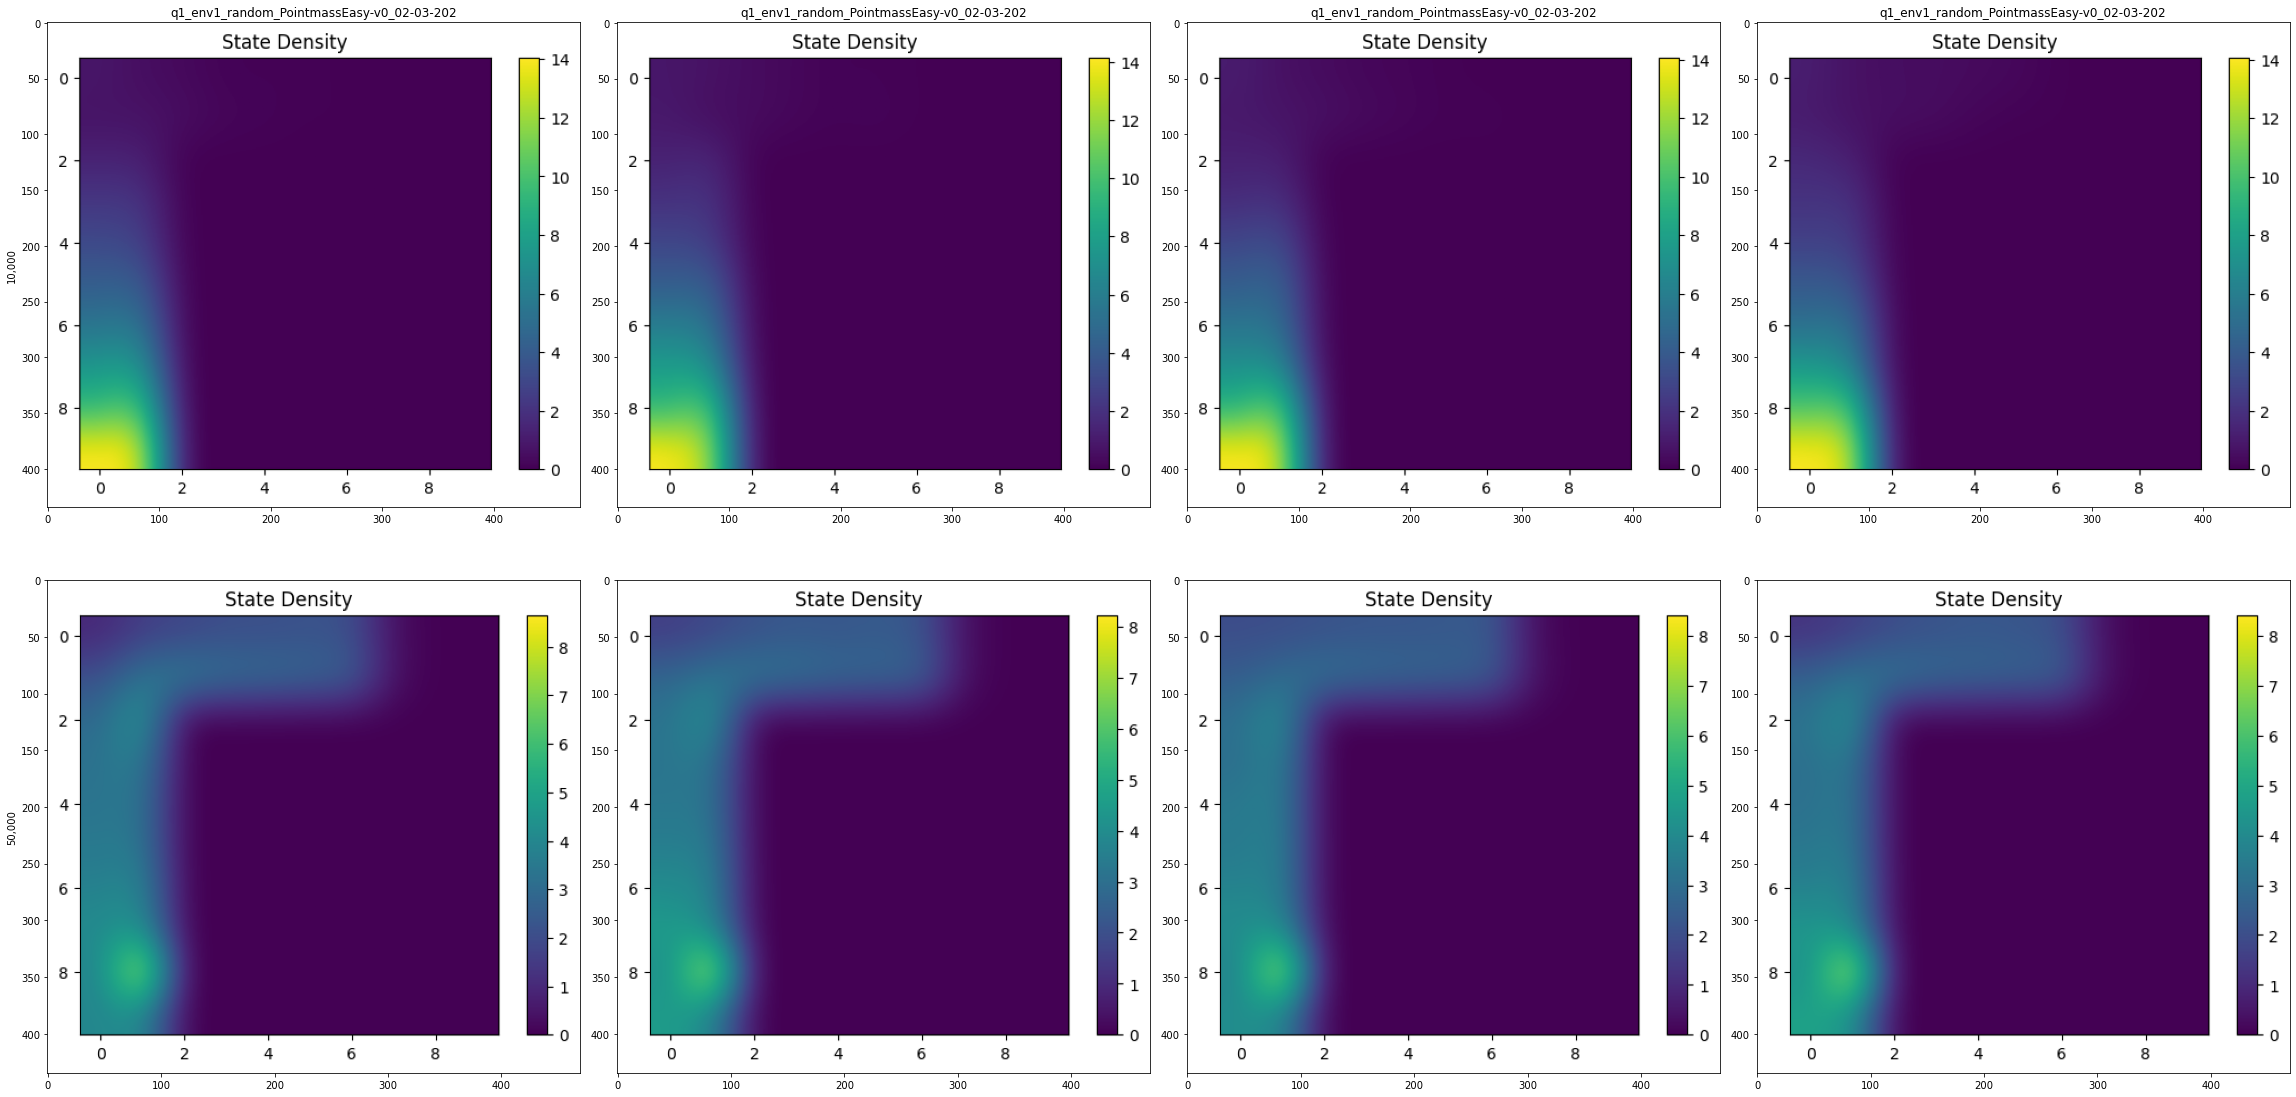
\includegraphics[scale=0.20]{p1/q1-easy-state-density-random}

    After 10K training steps, state density for the random strategy seems to be concentrated around the starting state and fades away as it moves away from the starting state.
    This is compatible with the expectation.

    \hspace*{-0.6in}
    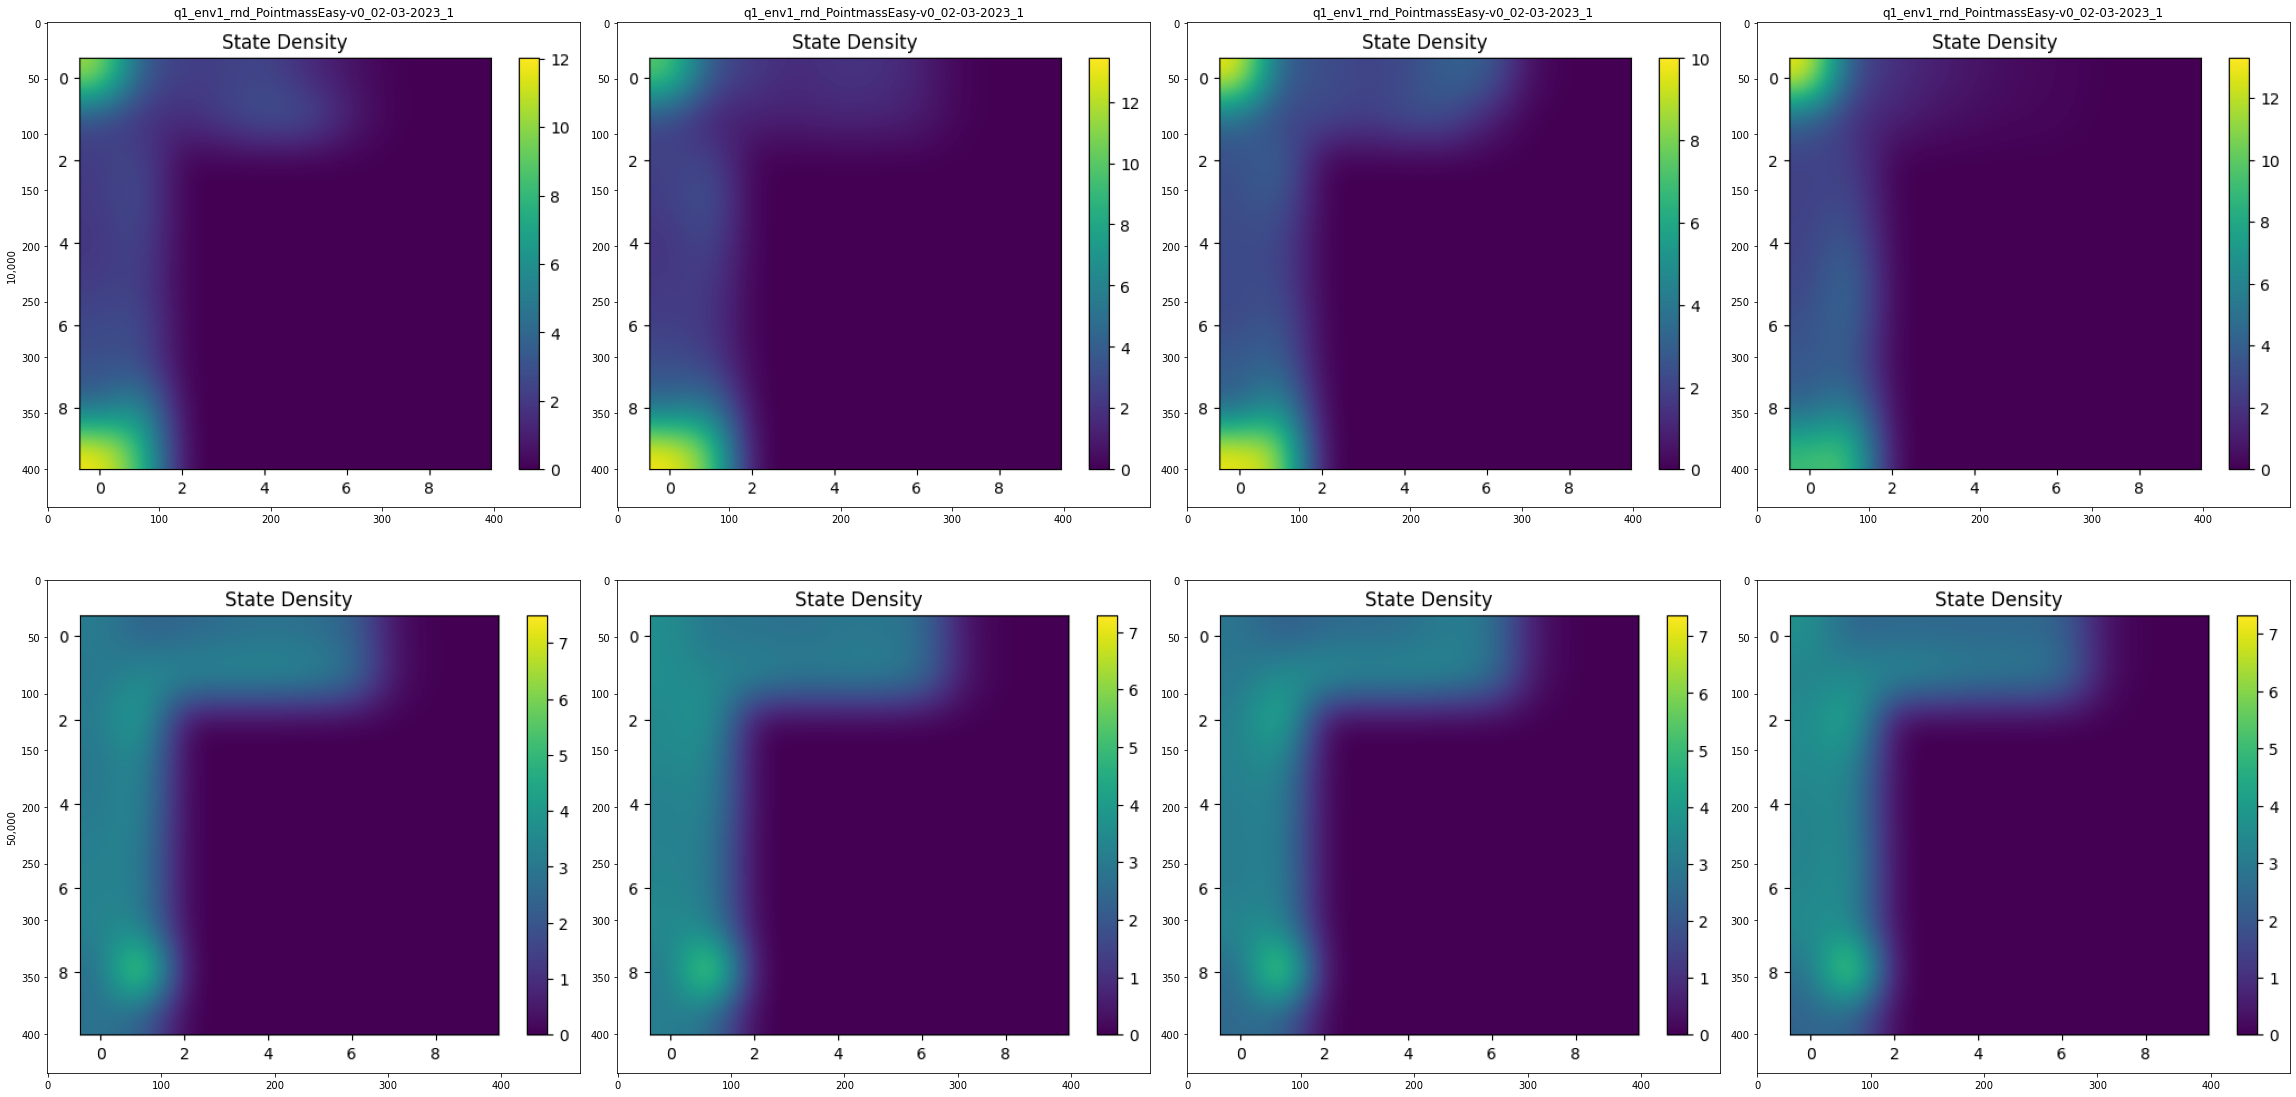
\includegraphics[scale=0.20]{p1/q1-easy-state-density-rnd}

    After 10K training steps, state density for the RND strategy seems to be more uniformly spread over the reachable parts of the environment.

    This is compatible with the expectation.

    After the online exploitation starts, state density becomes uniform over time.
    The difference between the two strategies disappears.

    \subsubsection{Medium Environment}

    \hspace*{-0.3in}
    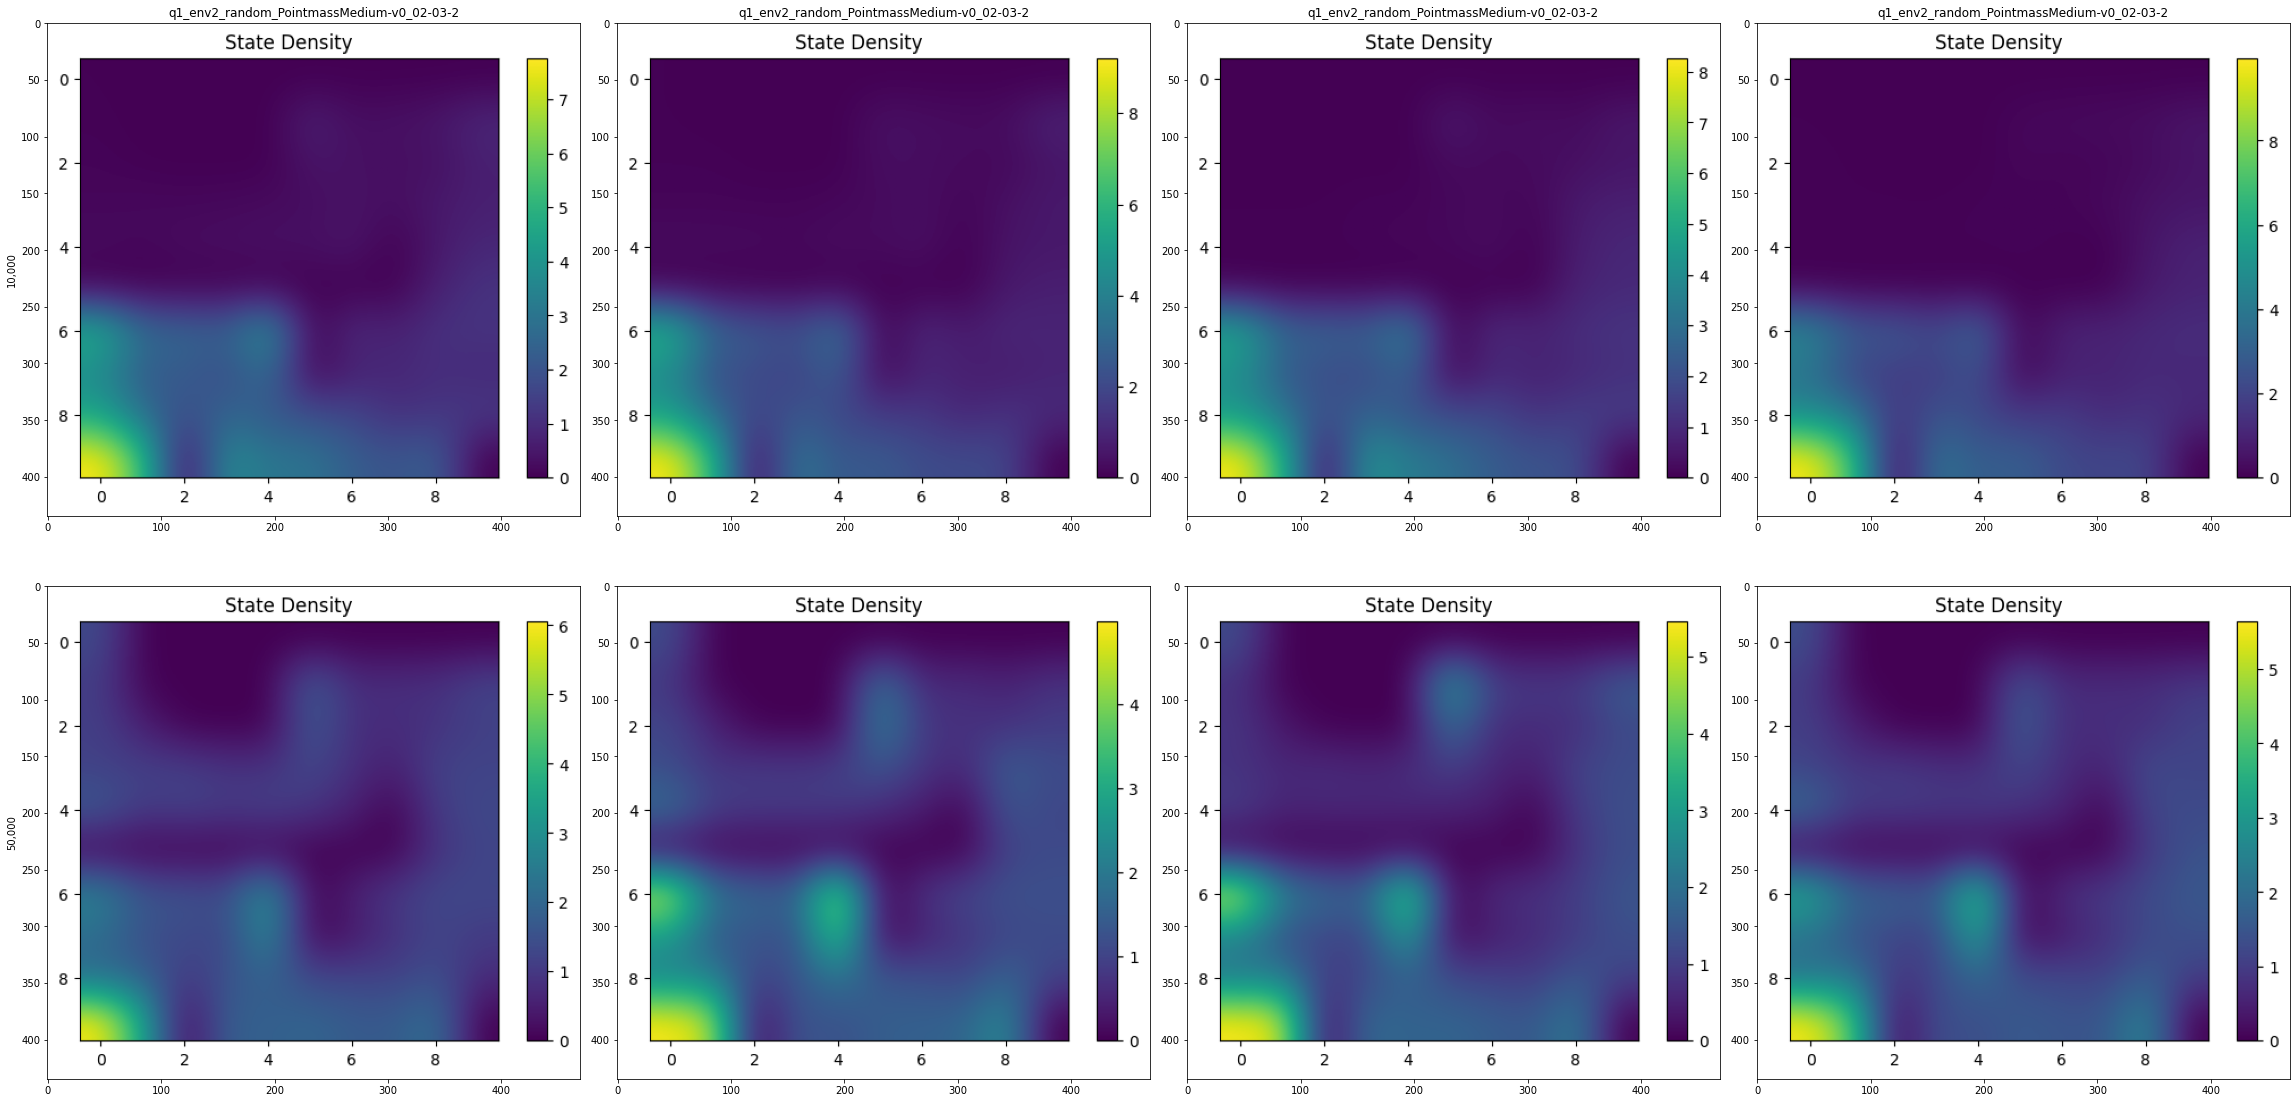
\includegraphics[scale=0.20]{p1/q1-medium-state-density-random}

    \hspace*{-0.6in}
    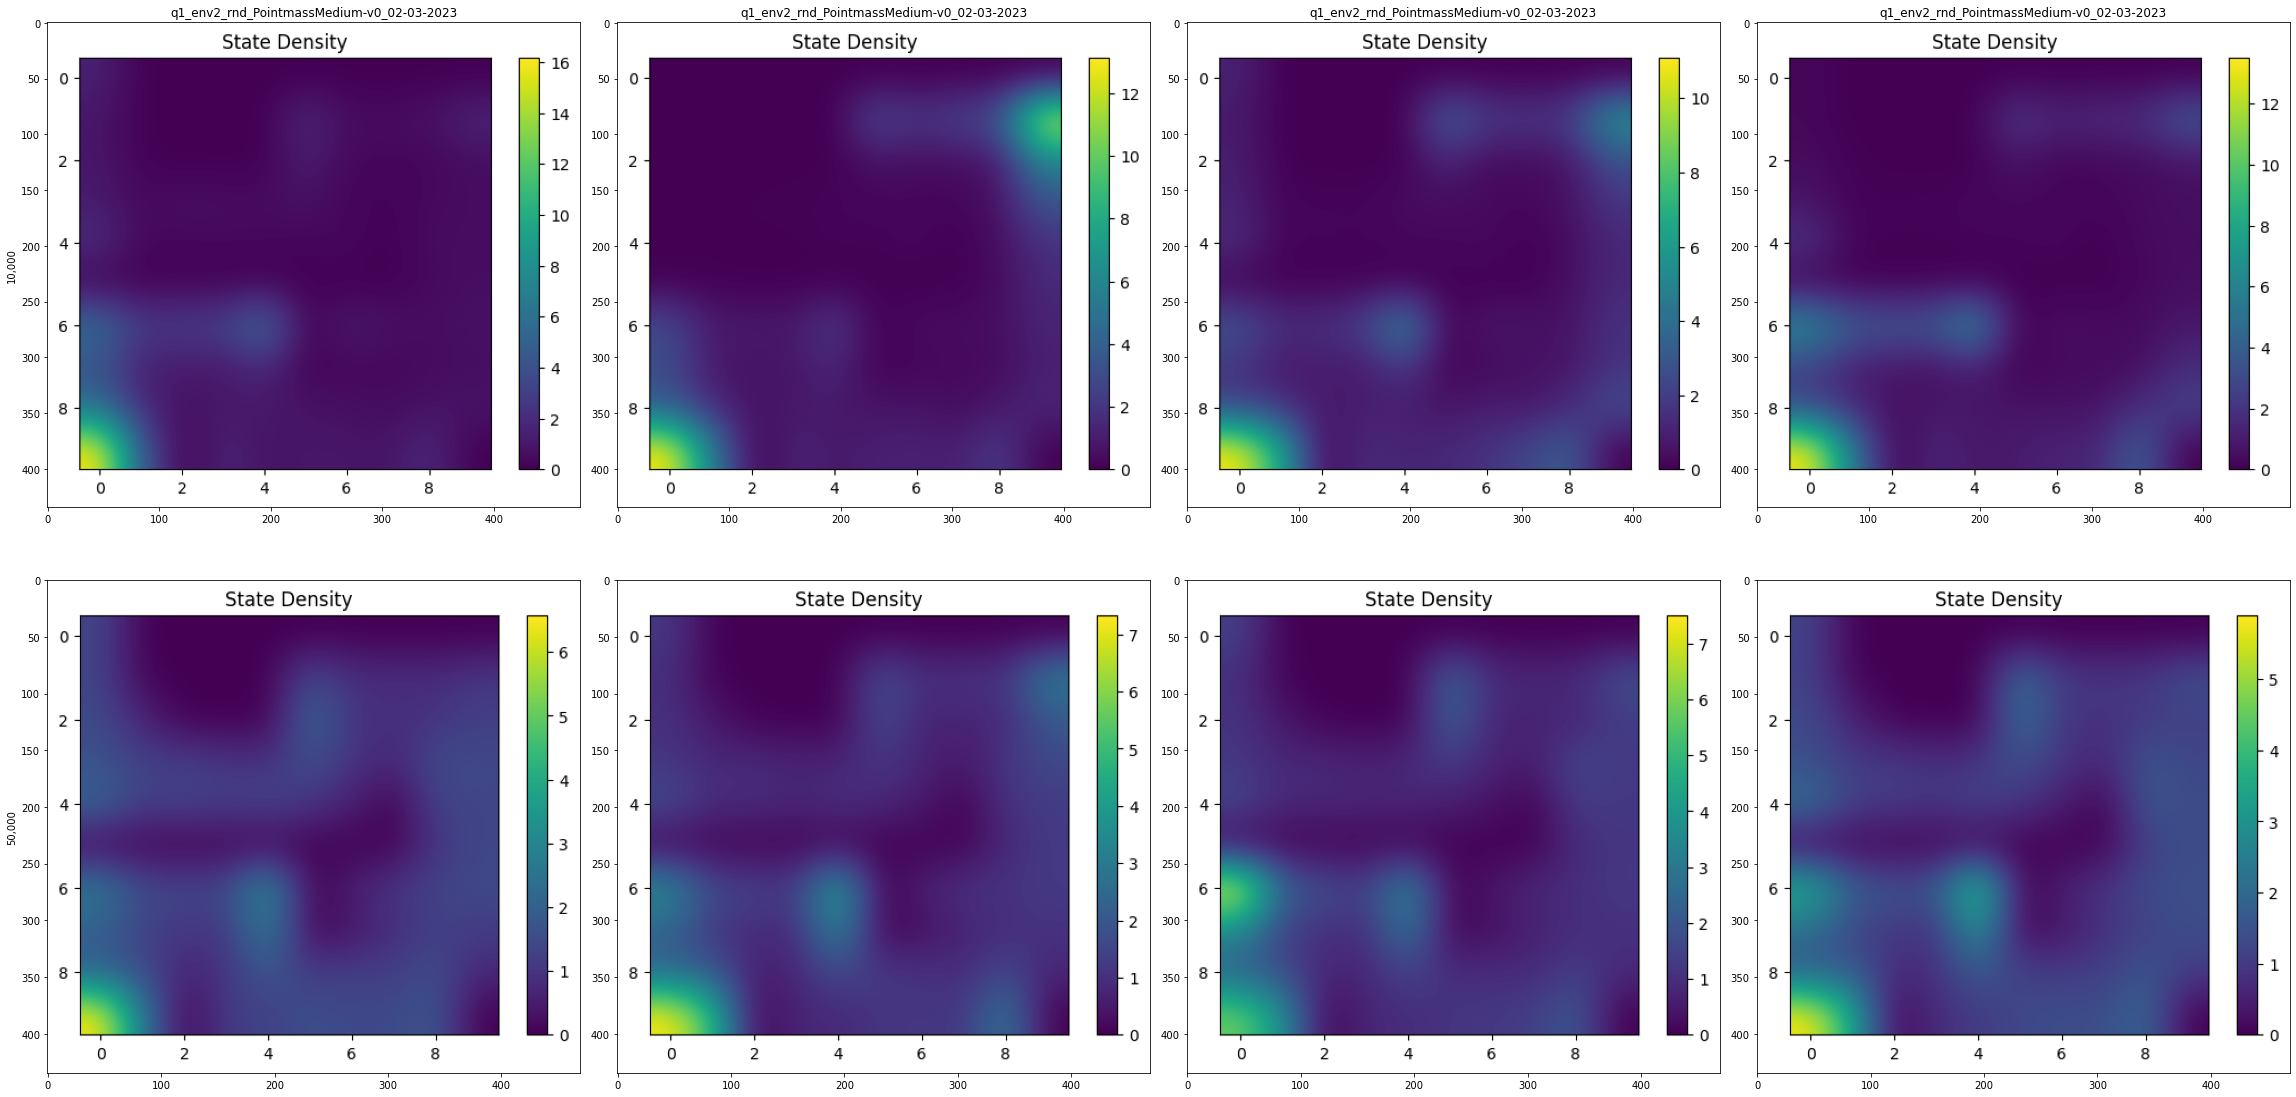
\includegraphics[scale=0.20]{p1/q1-medium-state-density-rnd}

    Until 10K steps, Random strategy generates state densities that are concentrated around the start state.
    Random strategy states density drops steadily as distance to start state increases.
    This behaviour is expected.

    RND strategy is expected to generate more uniform state densities, which seems not to be the case.
    10K state densities reaches up to 16 for RND strategy in comparison, Random strategy state densities reaches only up to 9.
    RND does better exploration by reaching the far side of the maze more often.

    After the online exploitation starts, state density becomes uniform over time.
    The difference between the two strategies disappears.

    \hspace*{-0.6in}
    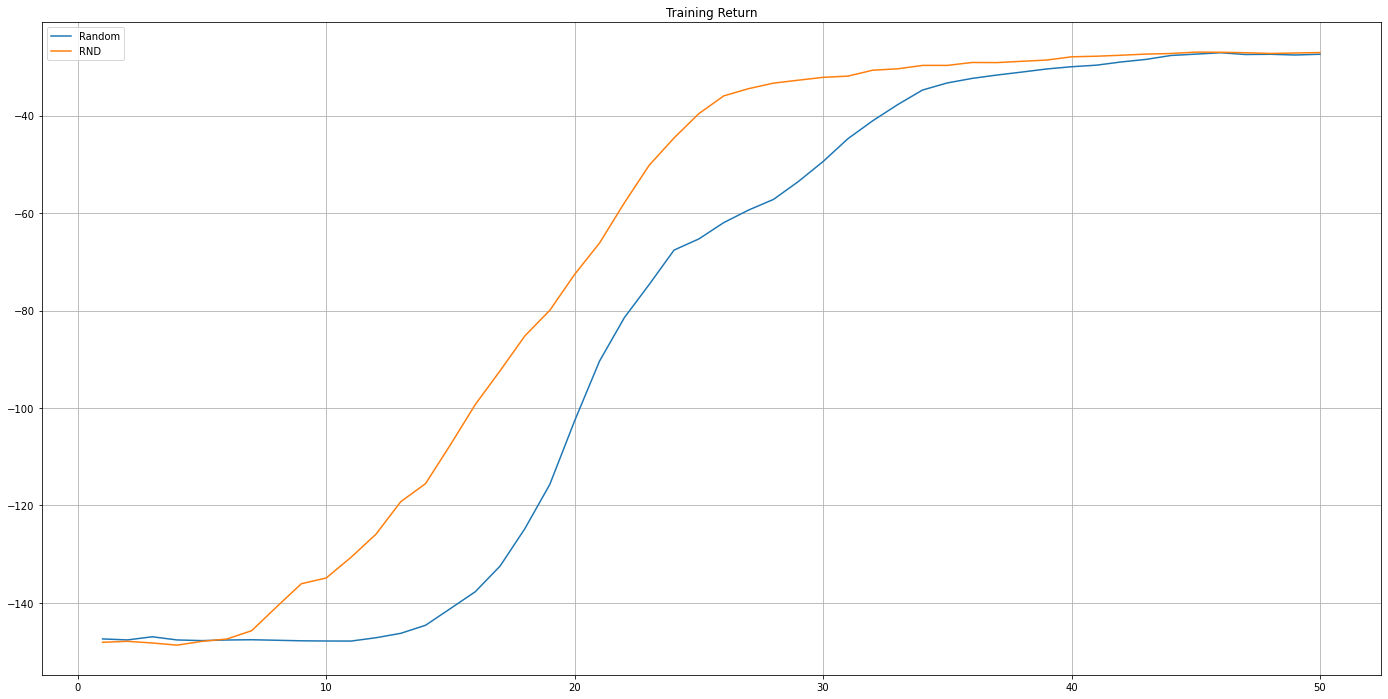
\includegraphics[scale=0.30]{q1/q1-medium-train-compare}

    RND strategy starts rising faster because it starts learning early.
    Random strategy then catch-ups.
    Performance is the same.

    \hspace*{-0.6in}
    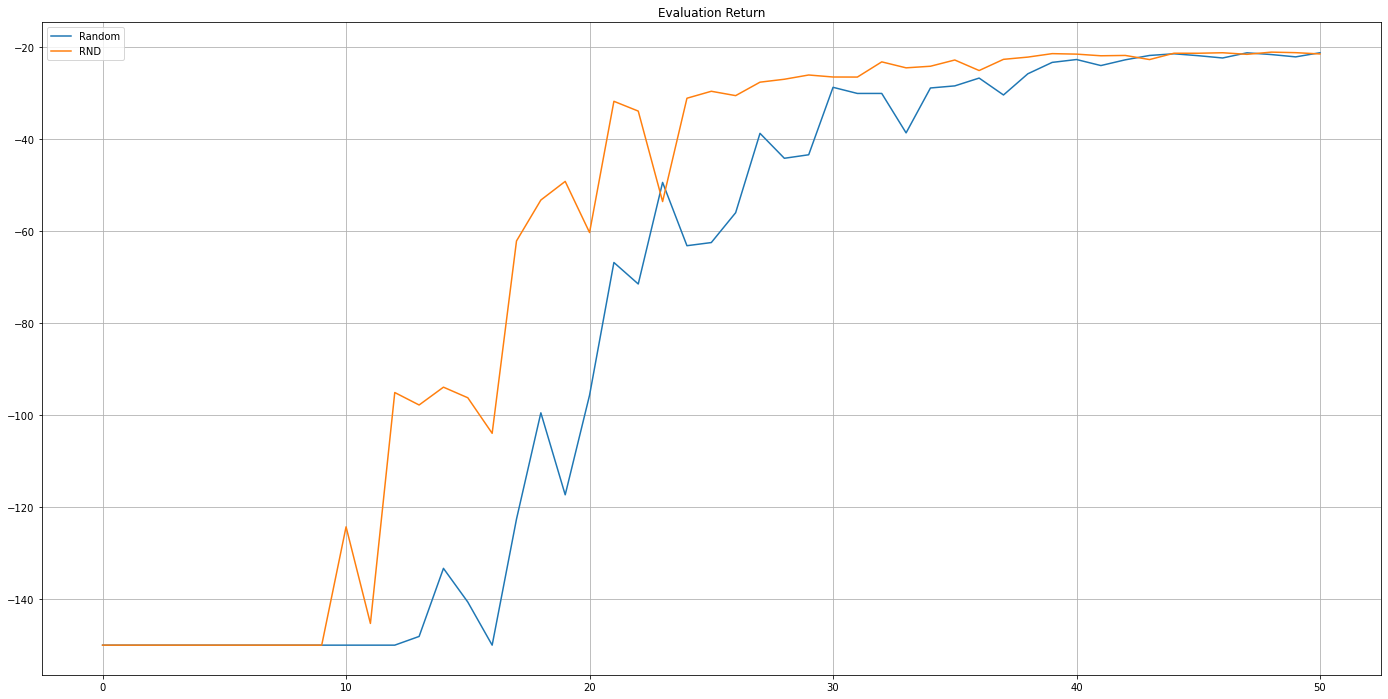
\includegraphics[scale=0.30]{q1/q1-medium-eval-compare}

    Evaluation performance follows the same discussions made for the training performance.

    \subsubsection{Hard Environment}

    \hspace*{-0.3in}
    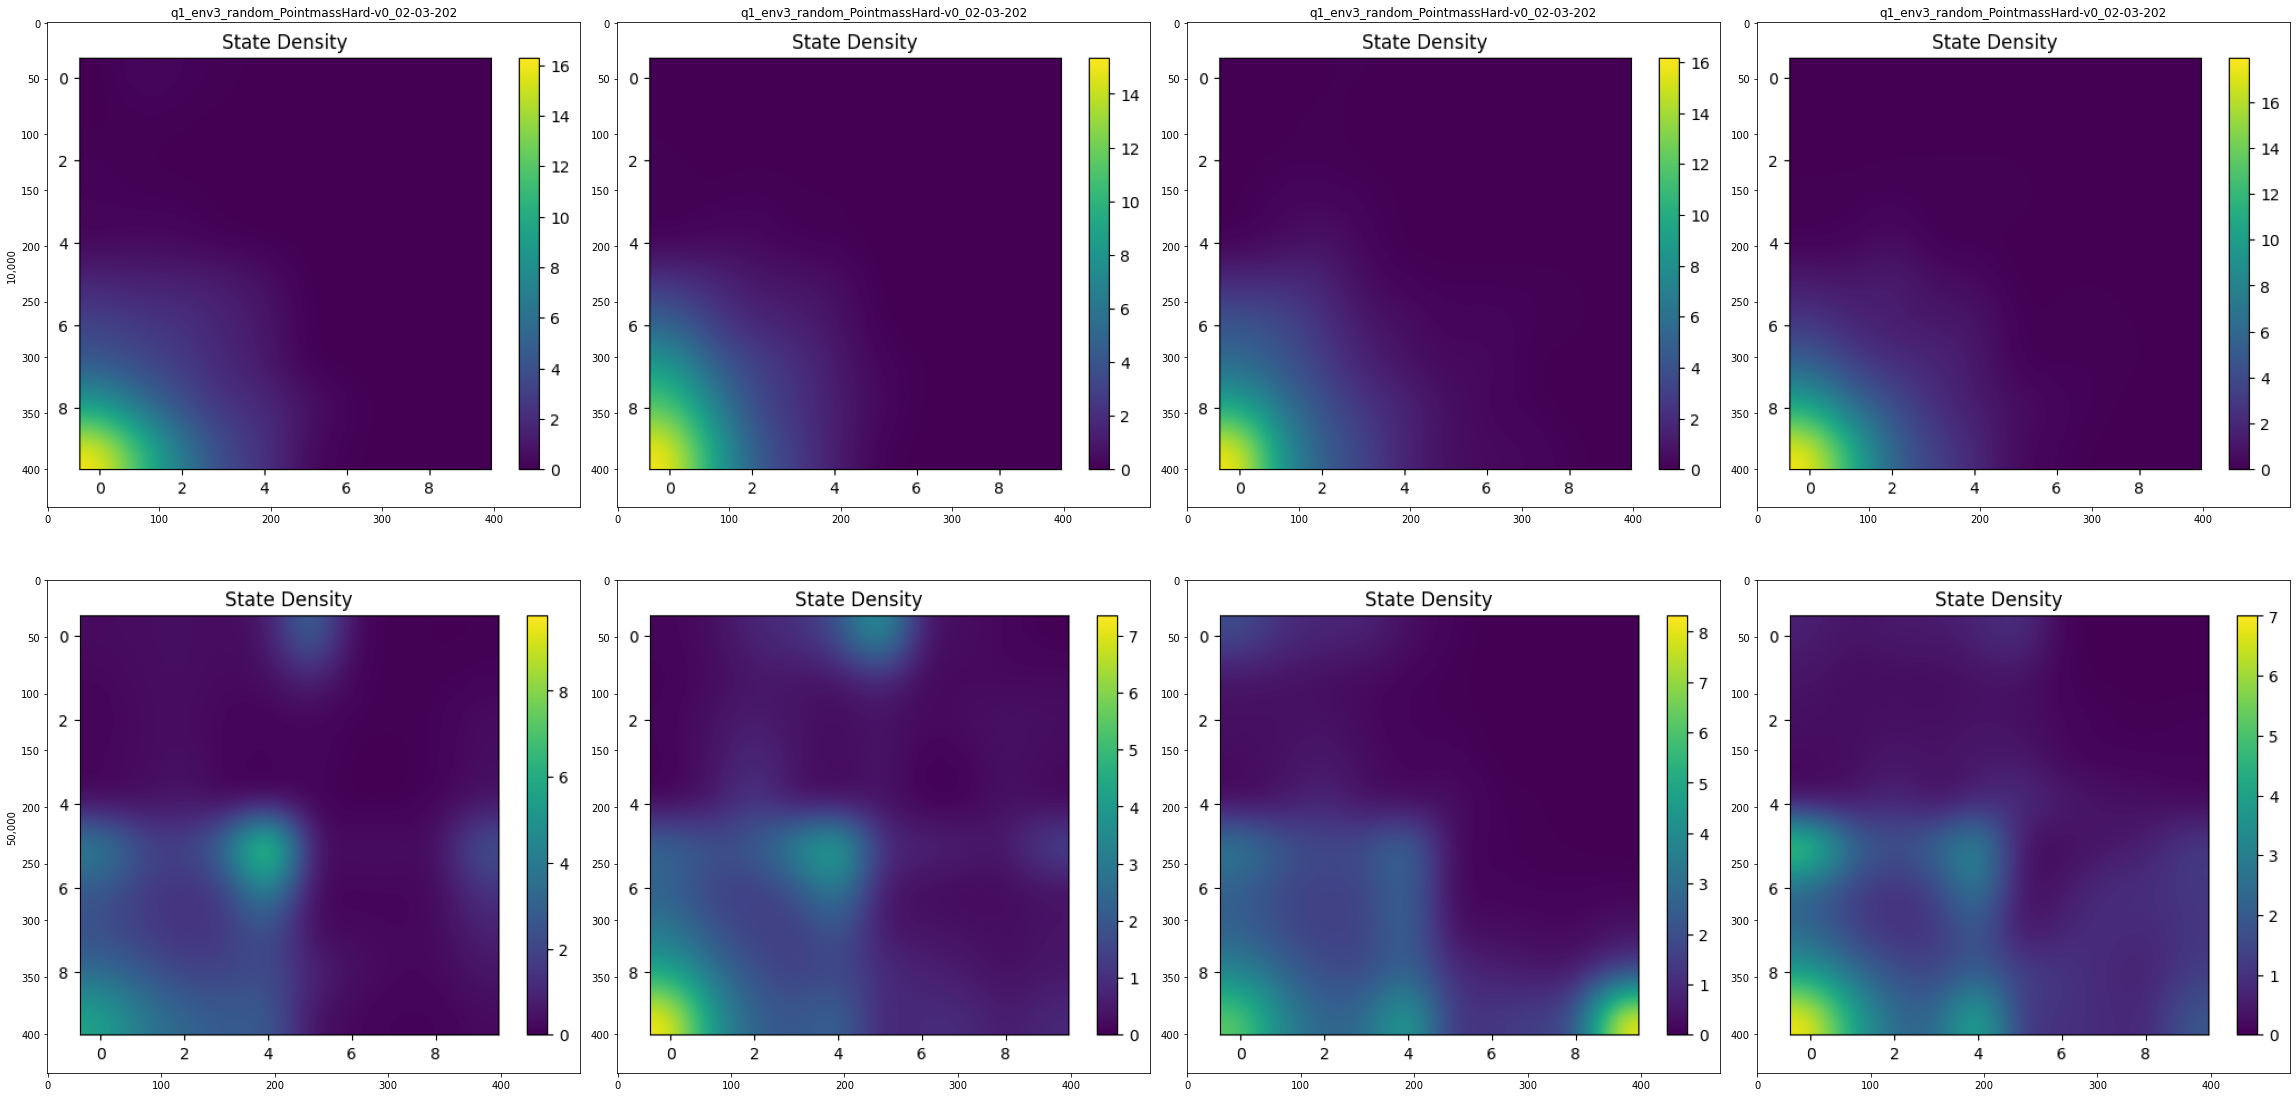
\includegraphics[scale=0.20]{p1/q1-hard-state-density-random}

    \hspace*{-0.6in}
    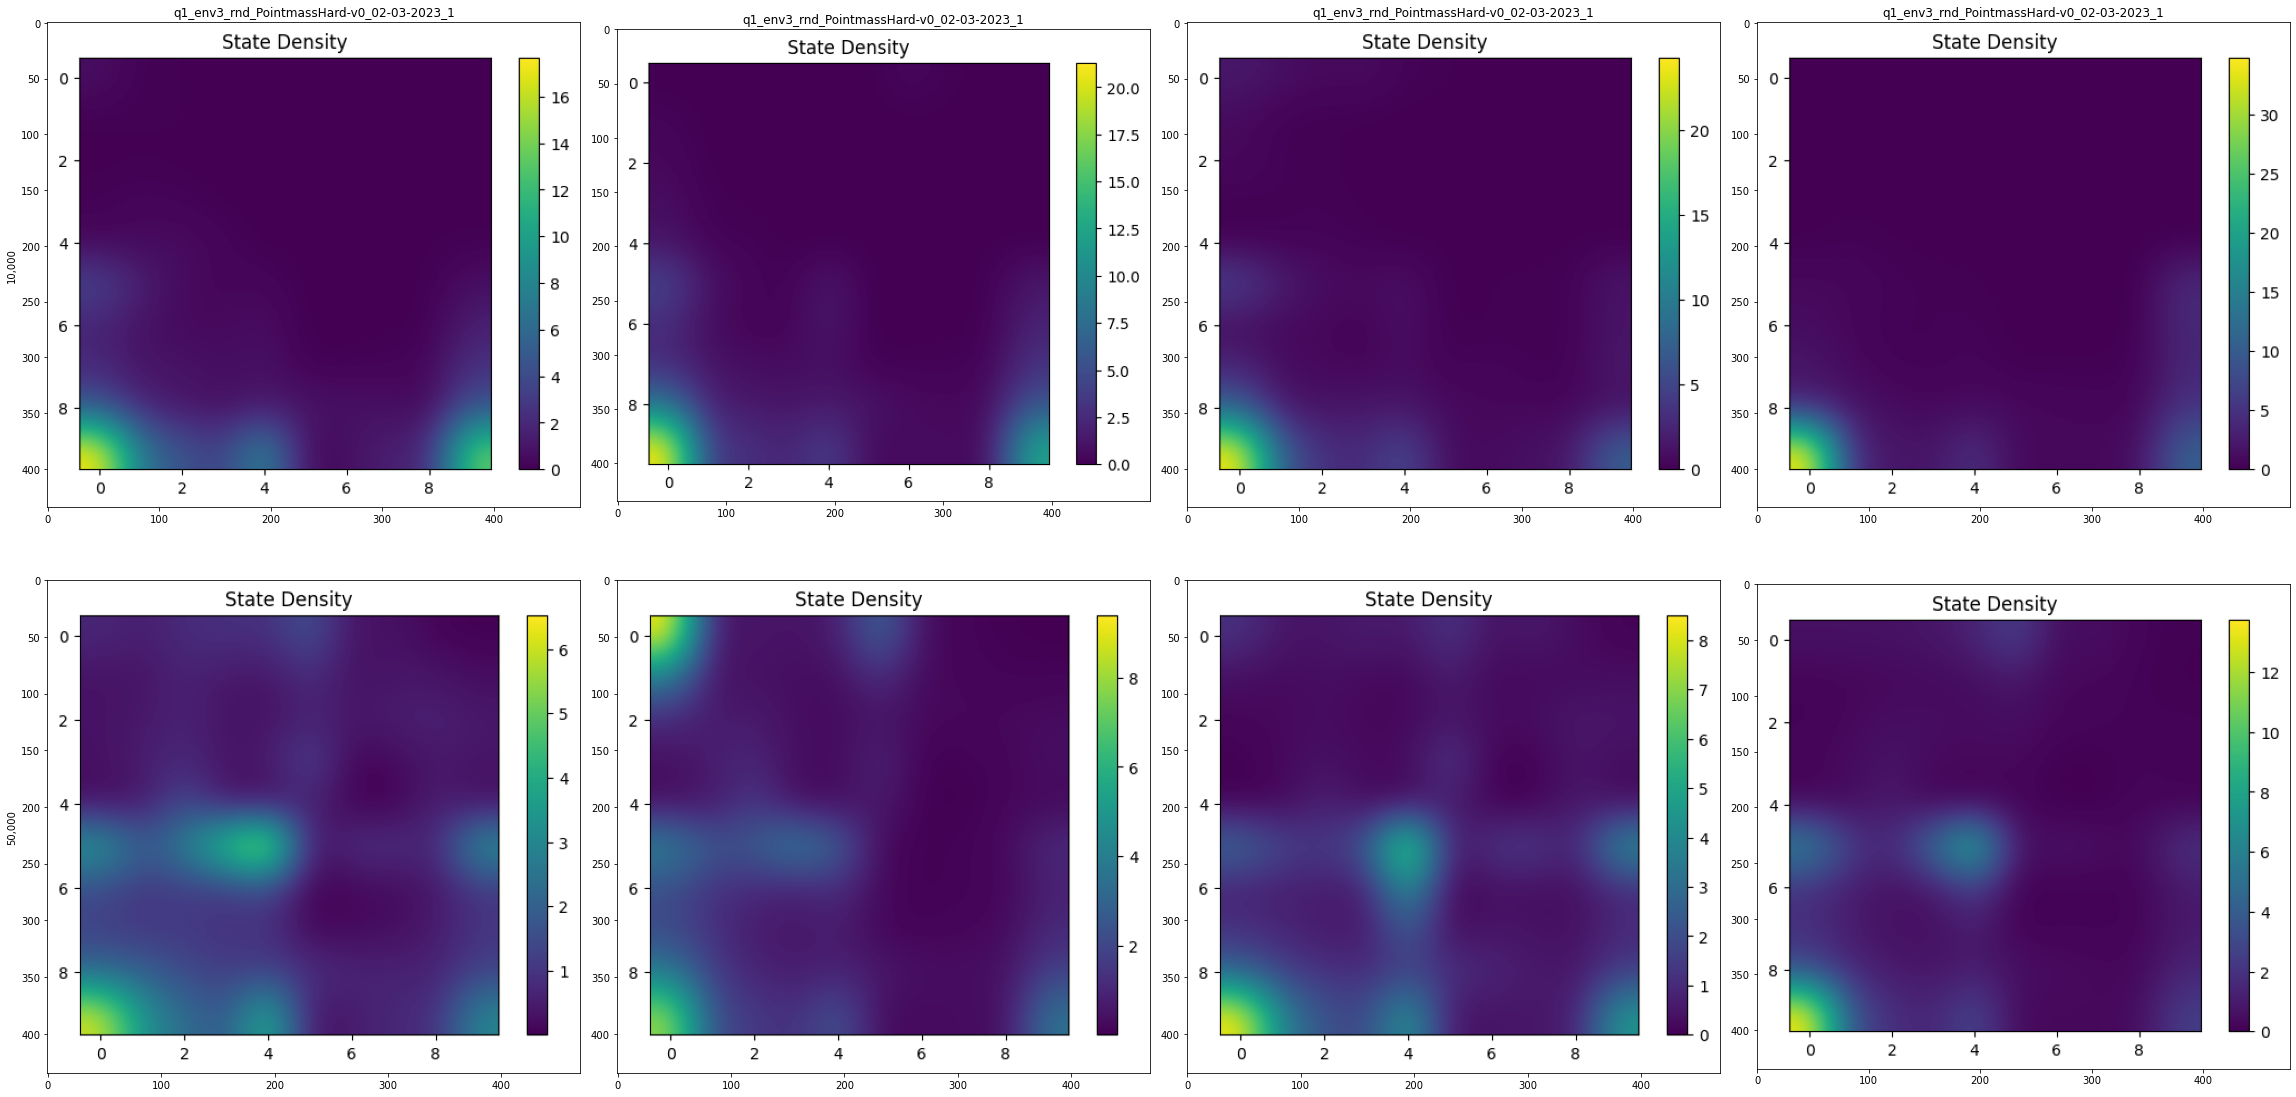
\includegraphics[scale=0.20]{p1/q1-hard-state-density-rnd}

    State densities follows the same discussions as the medium environment.

    \hspace*{-0.6in}
    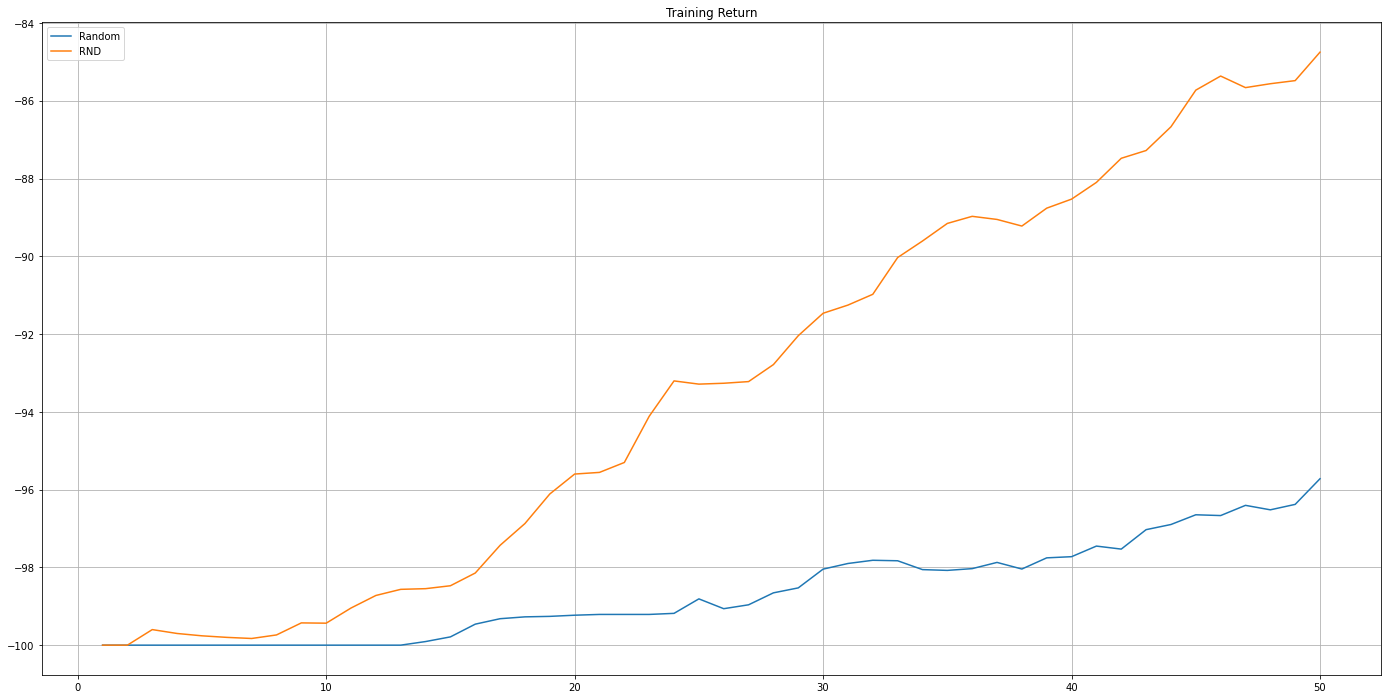
\includegraphics[scale=0.30]{p1/q1-hard-train-compare}

    \hspace*{-0.6in}
    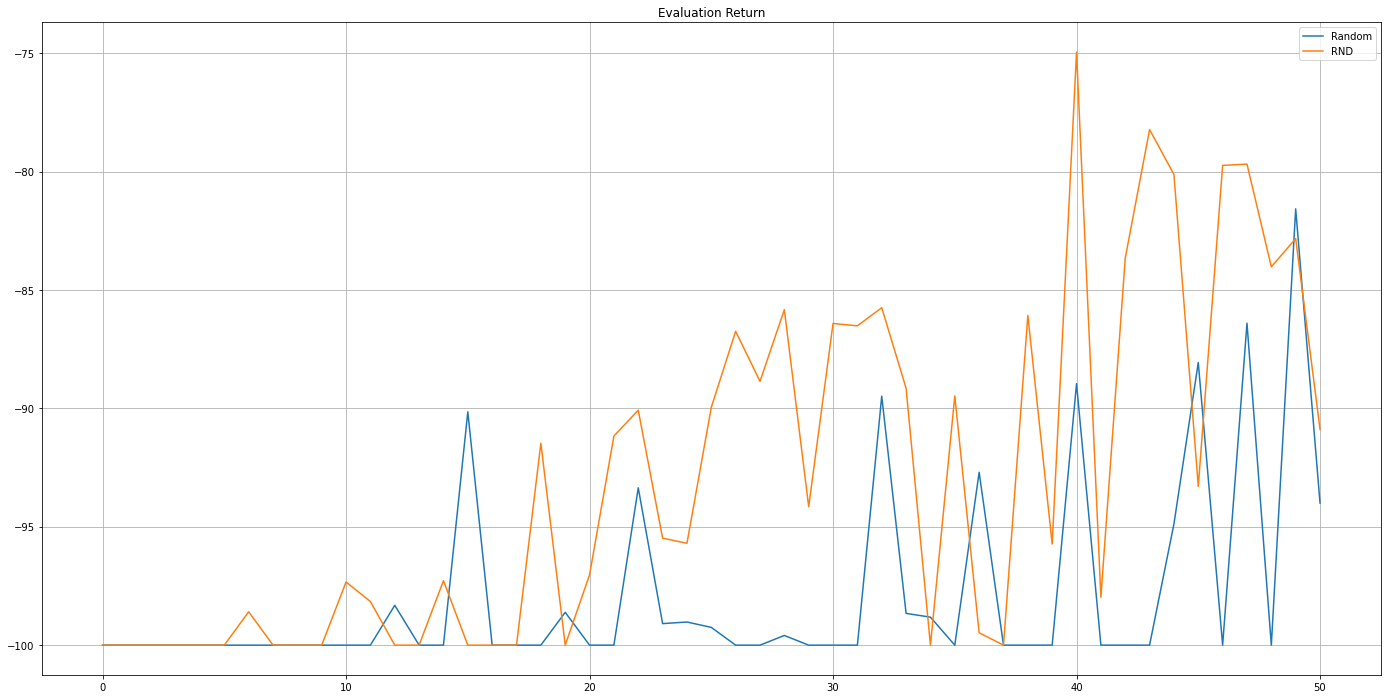
\includegraphics[scale=0.30]{p1/q1-hard-eval-compare}

    RND strategy performs better.
    In training, the gap between RND and Random keeps widening.
    In evaluation, the gap tends to close and random catches the RND by the end of the training.

    \subsection{Count Based Exploration Implementation}

    Target environment is a simple 2D environment.
    A simple count based exploration strategy can be used.

    A state representation consists two features each in the range of 0-1.
    State aggregation can be used to decrease number of states.
    0-1 range is discretized into 50 parts.
    Counts are kept in the discretized space.
    Count table consists of 2500 elements.
    Each table element is initialized to 1.

    Count based exploration strategy is implemented in a similar way to RND strategy.
    So results are expected to be at least as good as RND strategy.

    During training, state S is discretized into s.
    At each training step count for state s is increased by 1.
    Exploration bonus is calculated as 1/CNT(s) where CNT(s) gives the count for the discretized state s.

    Count based exploration strategy is referred to as CNT in the following discussions.

    \subsubsection{Easy Environment}

    \hspace*{-0.3in}
    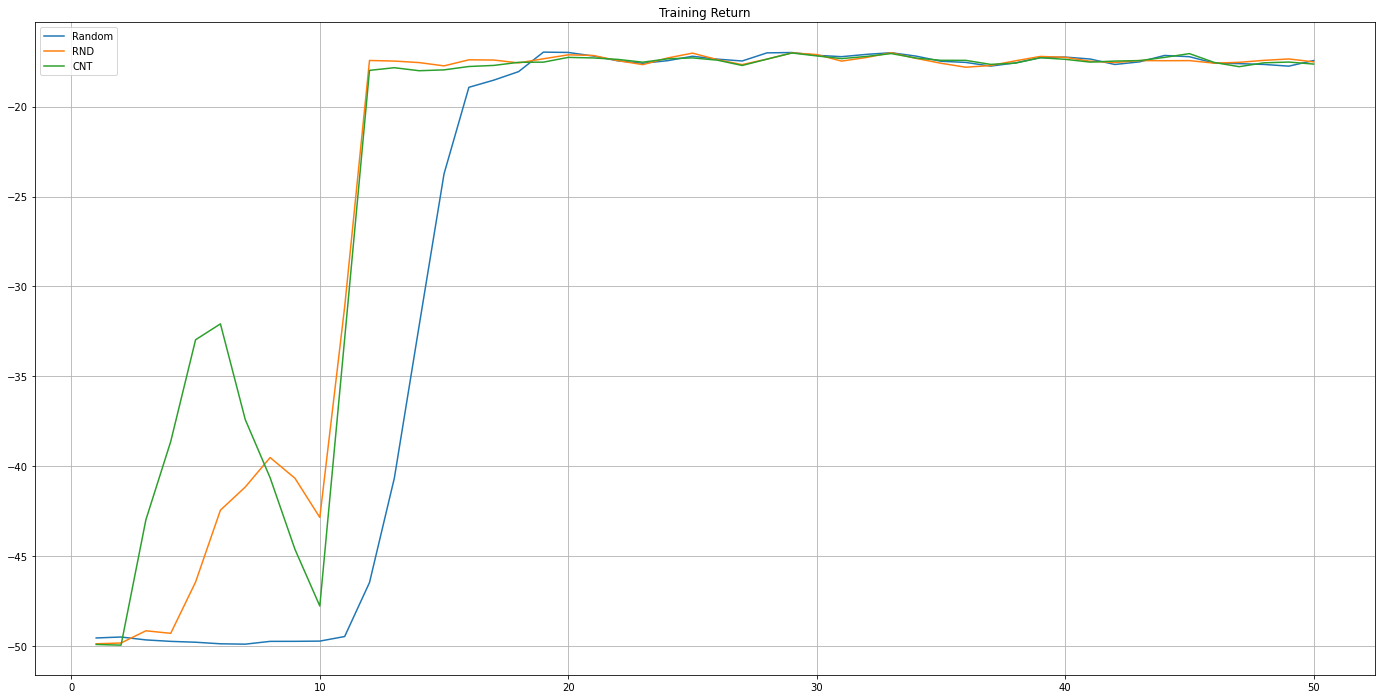
\includegraphics[scale=0.30]{p1/q1-p2-cnt-easy-train}

    \hspace*{-0.6in}
    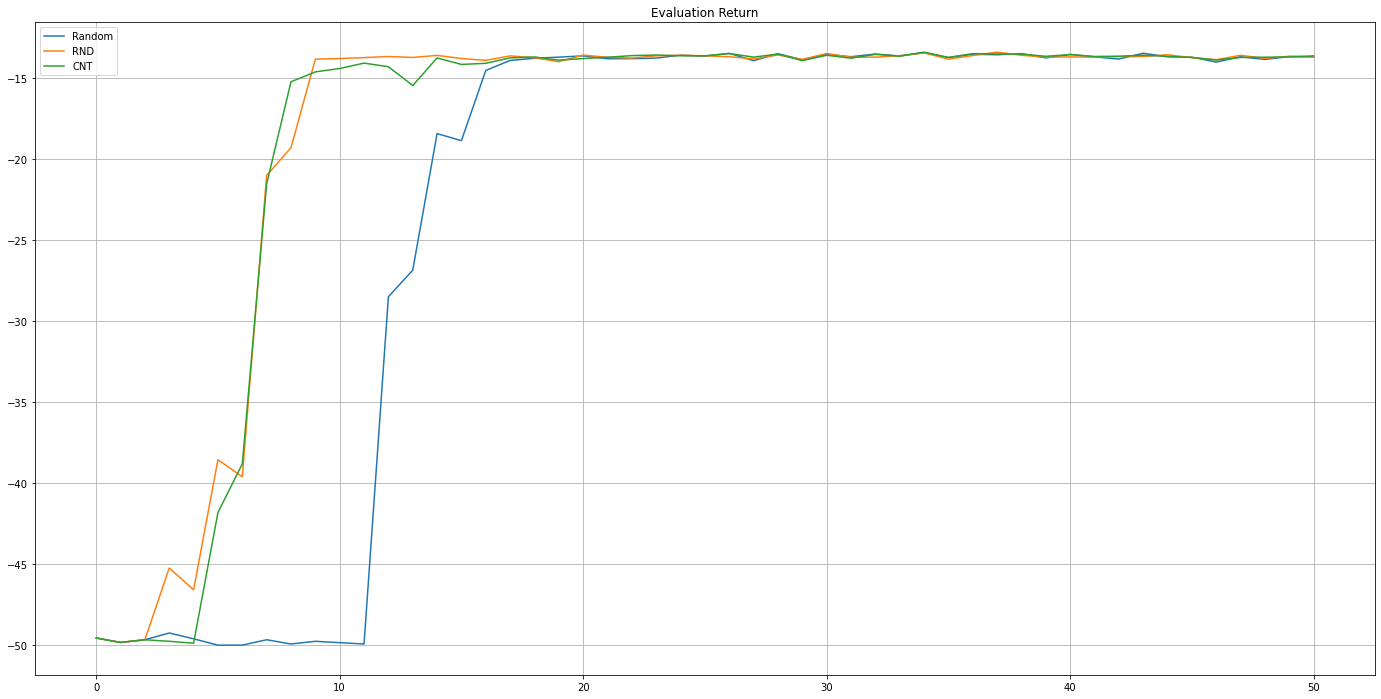
\includegraphics[scale=0.30]{p1/q1-p2-cnt-easy-eval}

    \hspace*{-0.6in}
    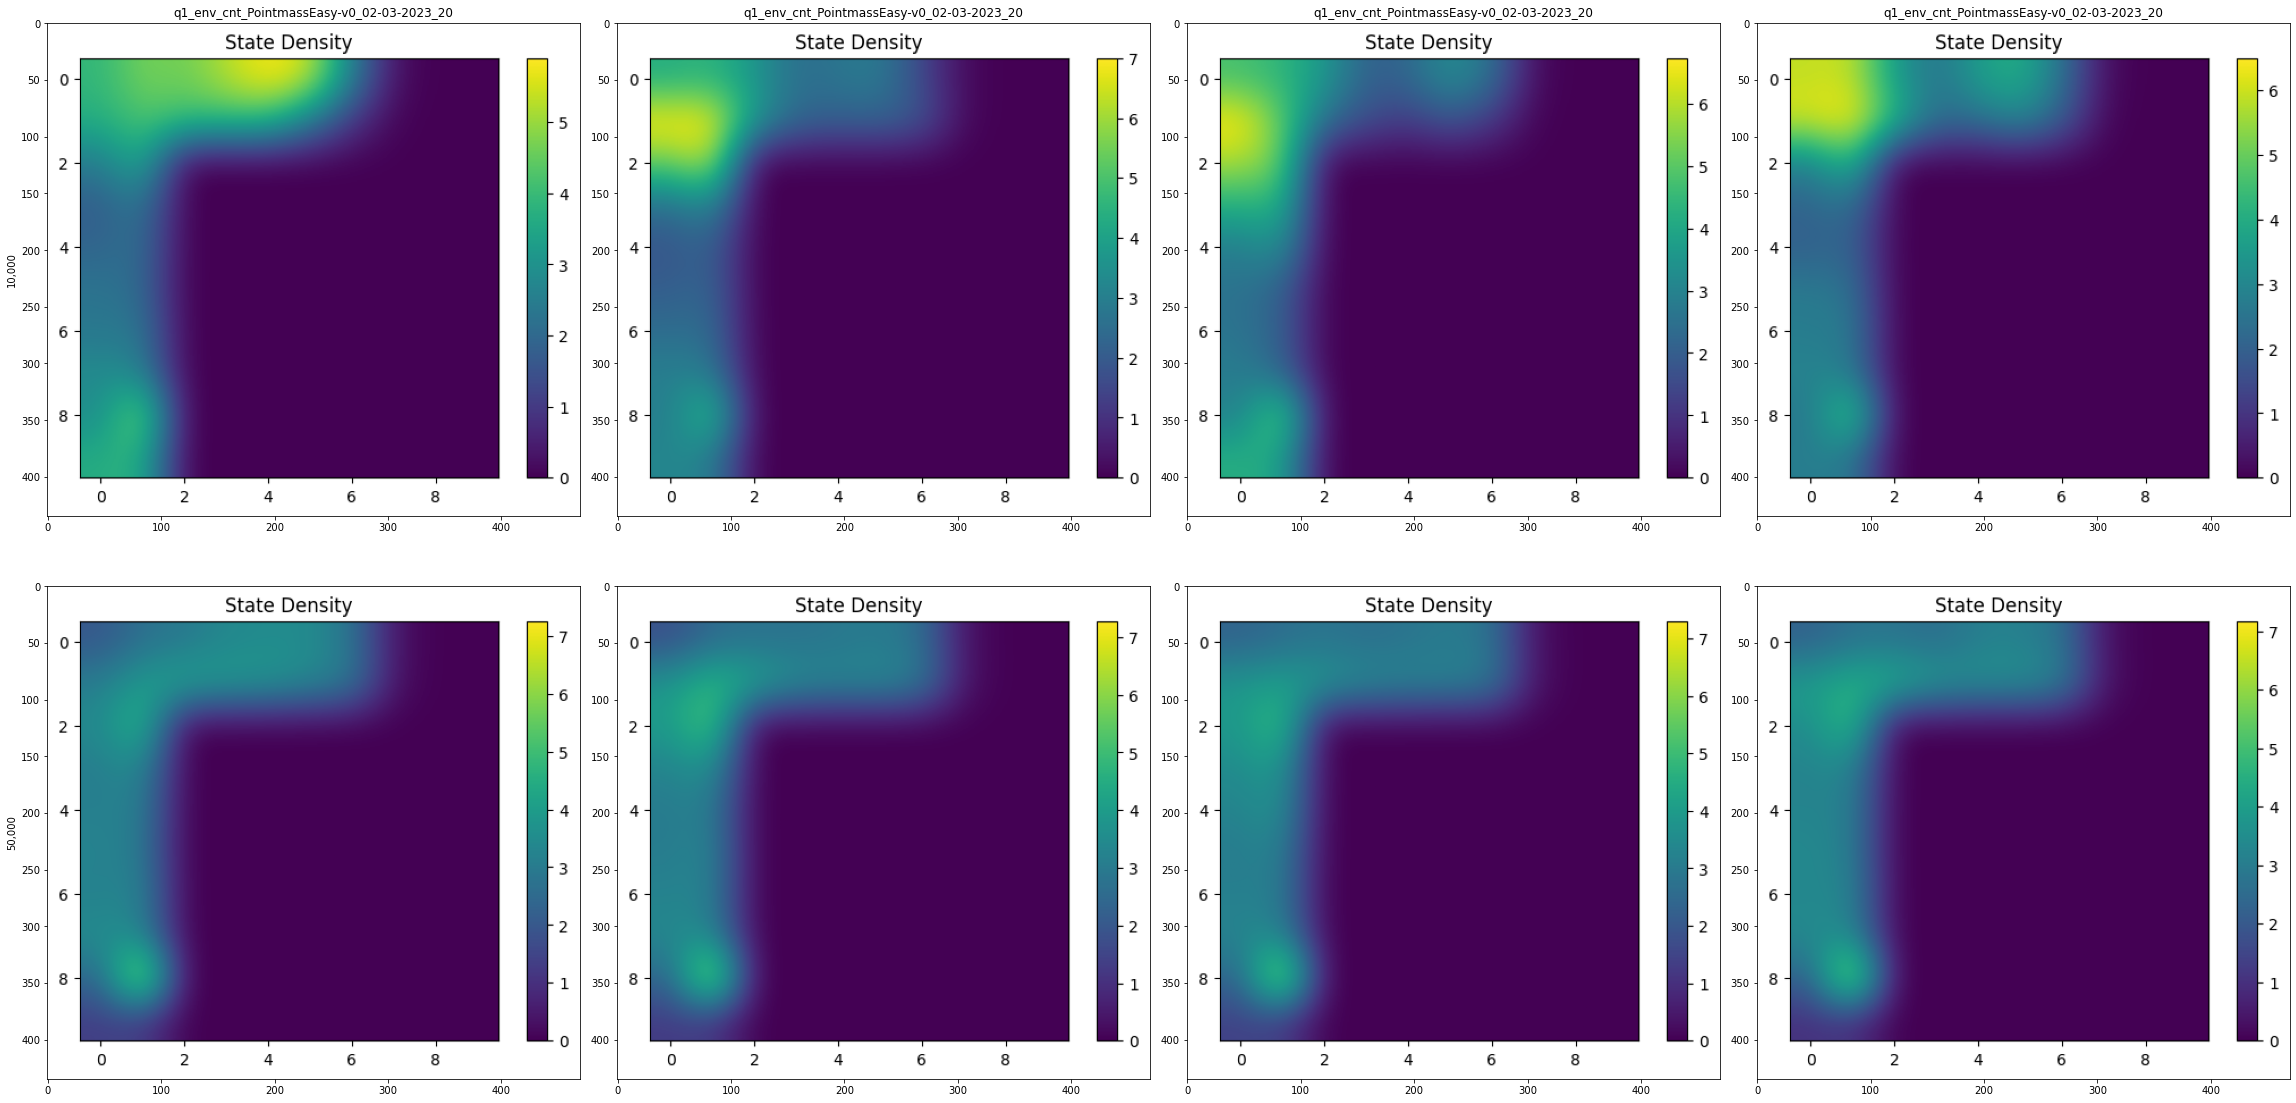
\includegraphics[scale=0.2]{p1/q1-p2-cnt-easy-state-density}

    Count based exploration strategy produces more uniform state densities than RND and Random strategies.
    In terms of training and evaluation performance CNT performs similar to RND strategy.
    In the easy environment difference is not distinguishable.

    \subsubsection{Medium Environment}

    \hspace*{-0.3in}
    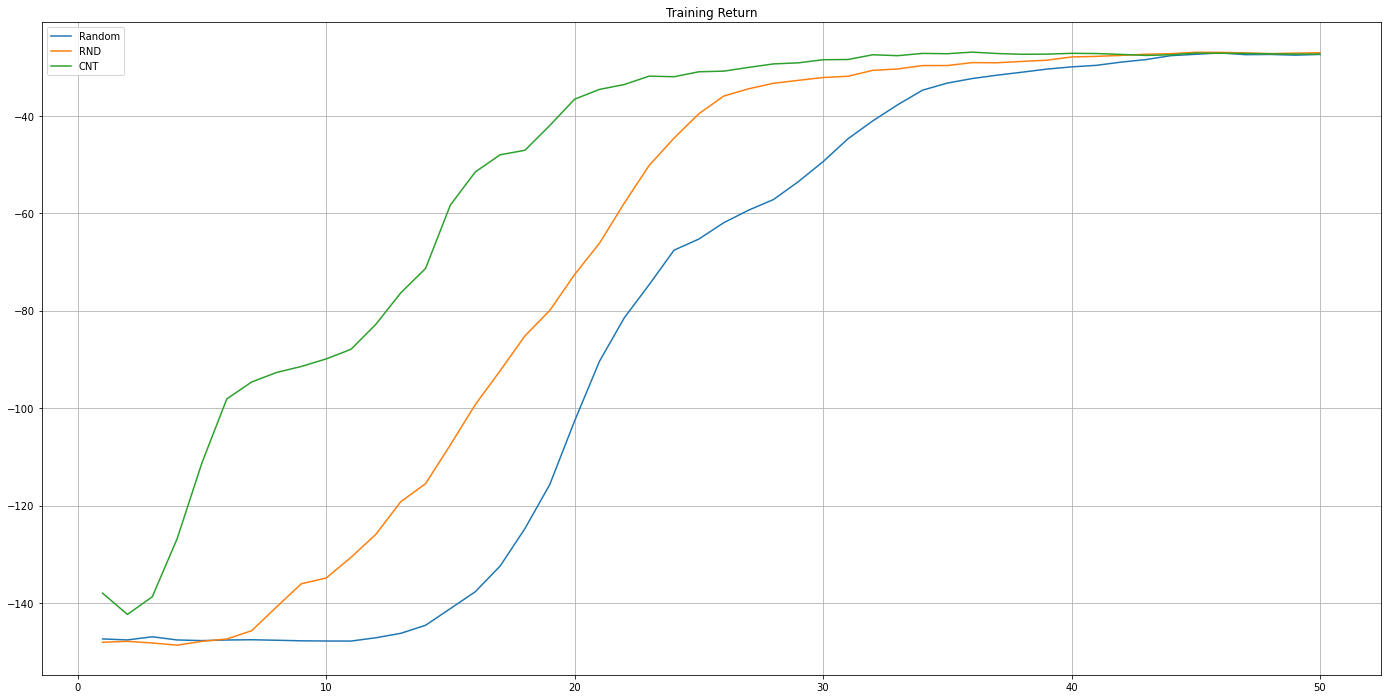
\includegraphics[scale=0.30]{p1/q1-p2-cnt-medium-train}

    \hspace*{-0.6in}
    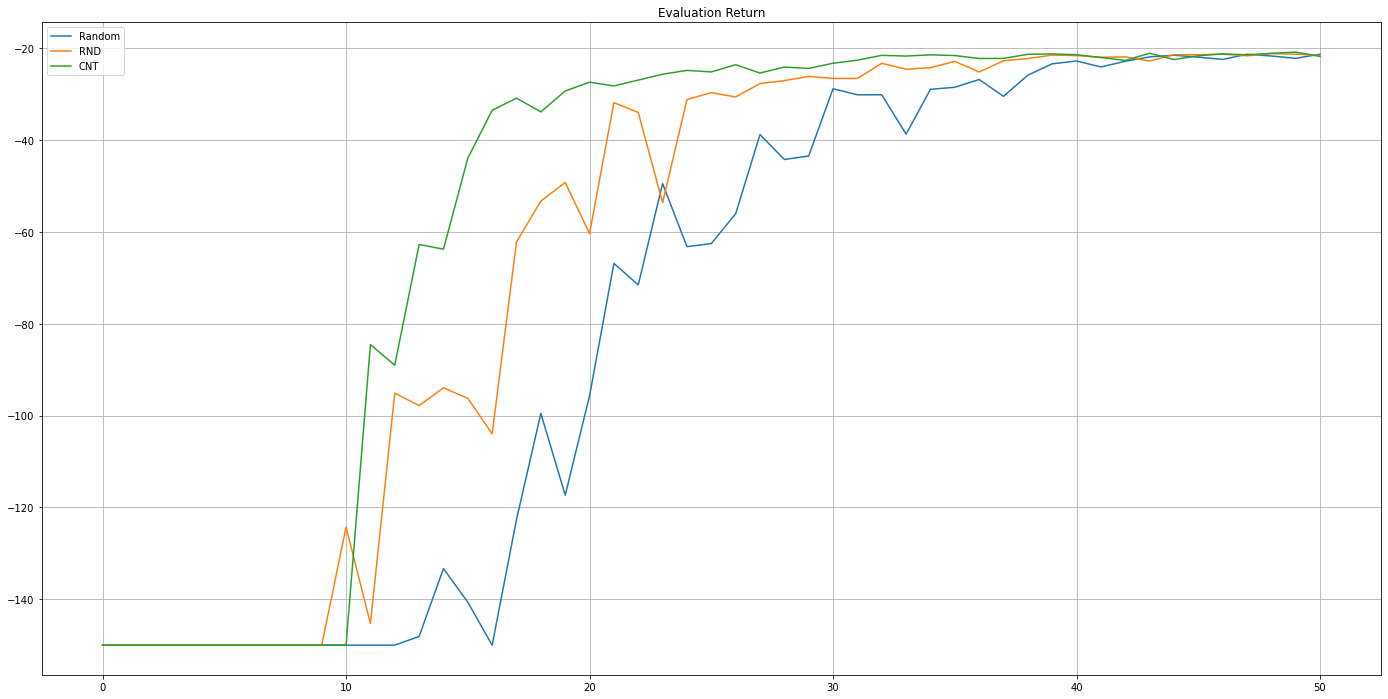
\includegraphics[scale=0.30]{p1/q1-p2-cnt-medium-eval}

    \hspace*{-0.6in}
    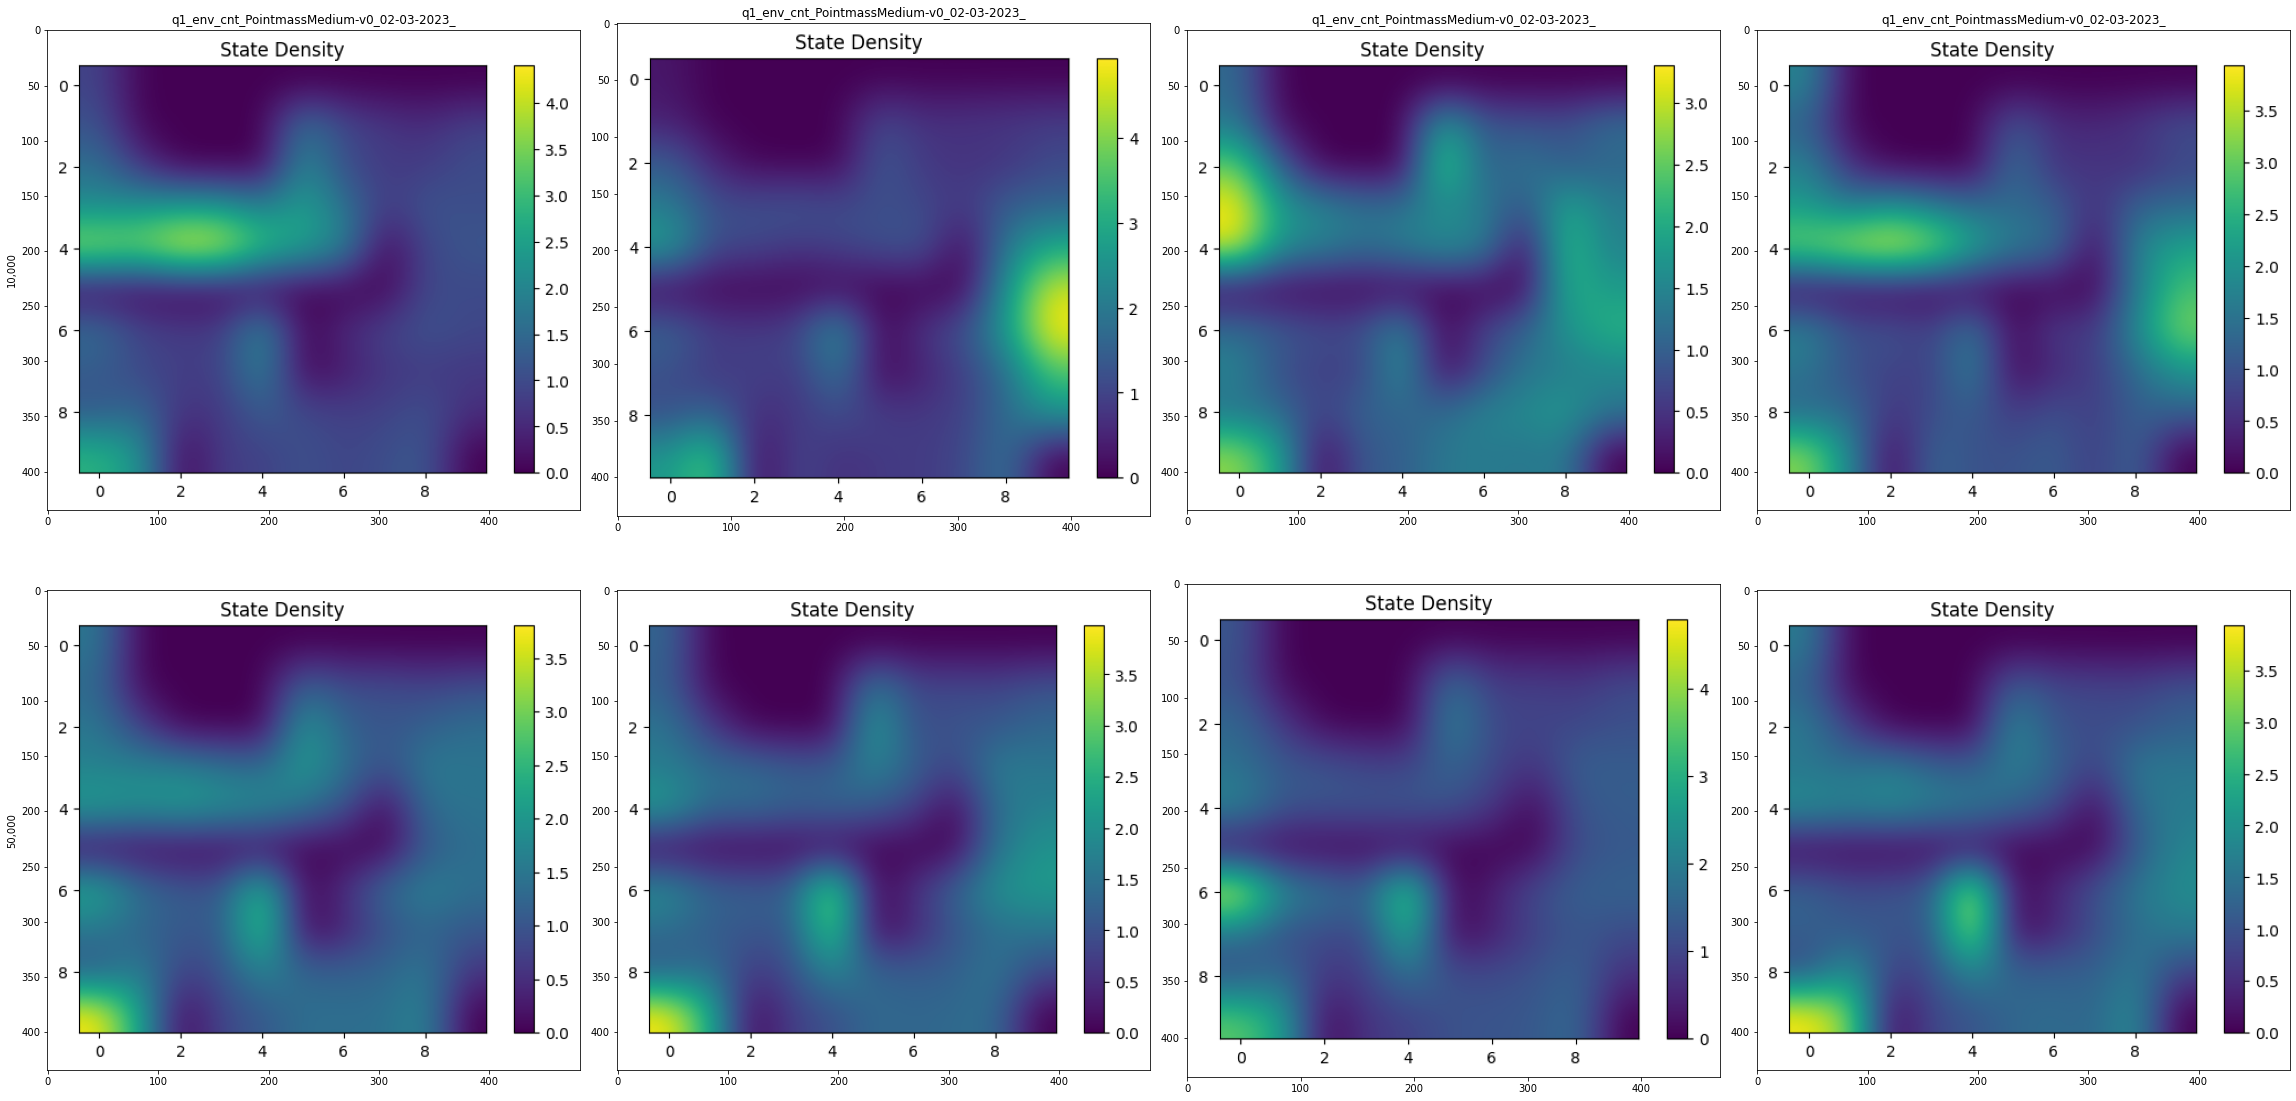
\includegraphics[scale=0.2]{p1/q1-p2-cnt-medium-state-density}

    Count based exploration strategy produces more uniform state densities than RND and Random strategies.
    In terms of training and evaluation performance CNT performs better than RND strategy.
    Performance difference is result of better exploration.

    \subsubsection{Hard Environment}

    \hspace*{-0.3in}
    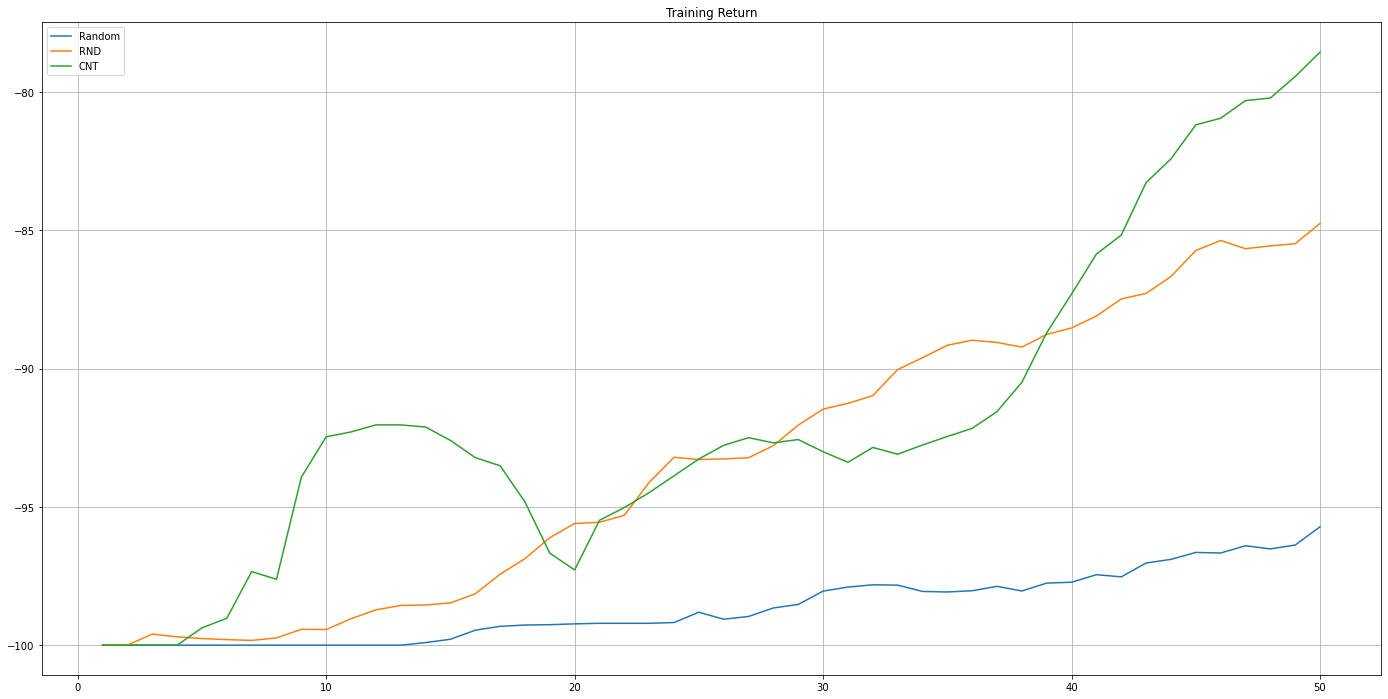
\includegraphics[scale=0.30]{p1/q1-p2-cnt-hard-train}

    \hspace*{-0.6in}
    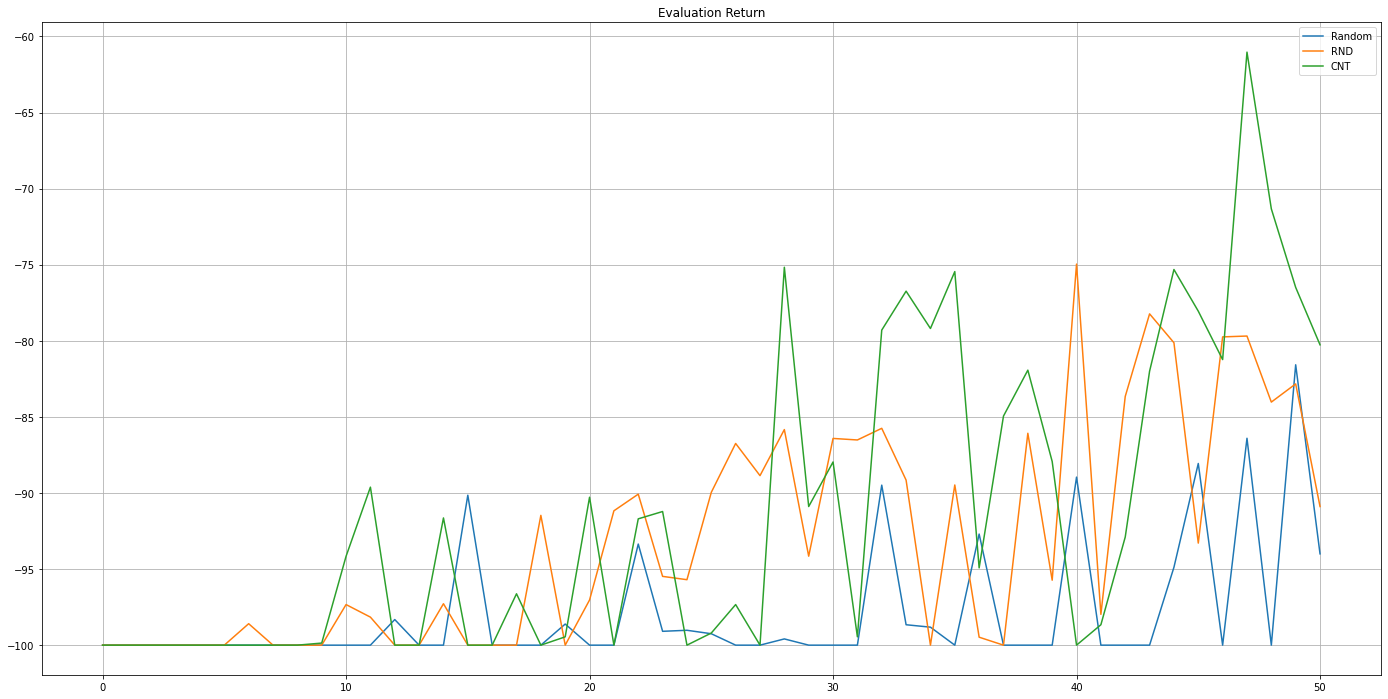
\includegraphics[scale=0.30]{p1/q1-p2-cnt-hard-eval}

    \hspace*{-0.6in}
    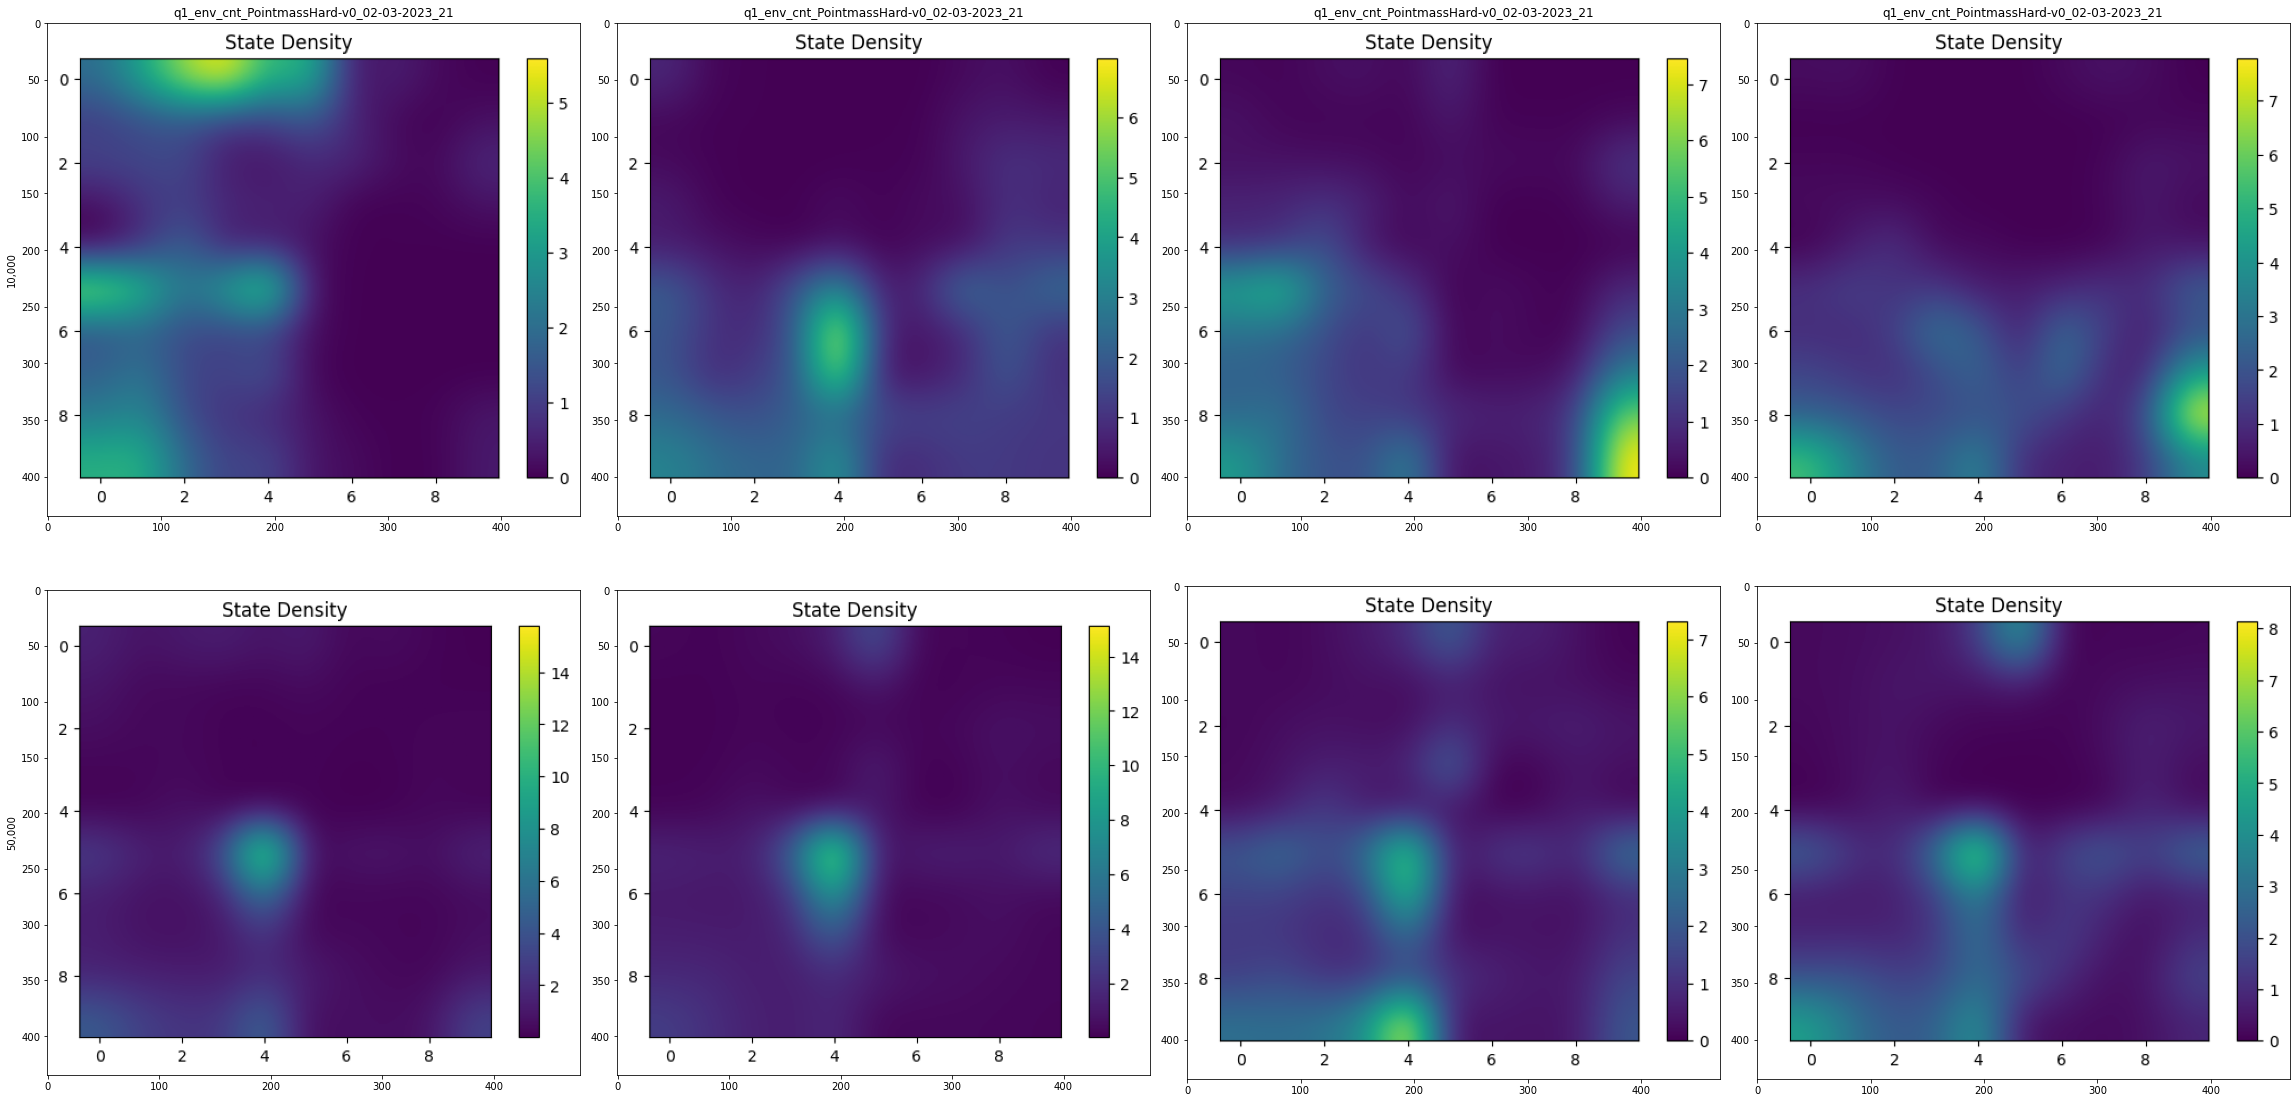
\includegraphics[scale=0.2]{p1/q1-p2-cnt-hard-state-density}

    Count based exploration strategy generates more uniform 10K state densities than RND.

    CNT training and evaluation performances are better than Random and RND strategy performances.


    \section{Part 2: Offline learning on exploration data}

    \subsection{DQN vs CQL}

    \hspace*{-0.6in}
    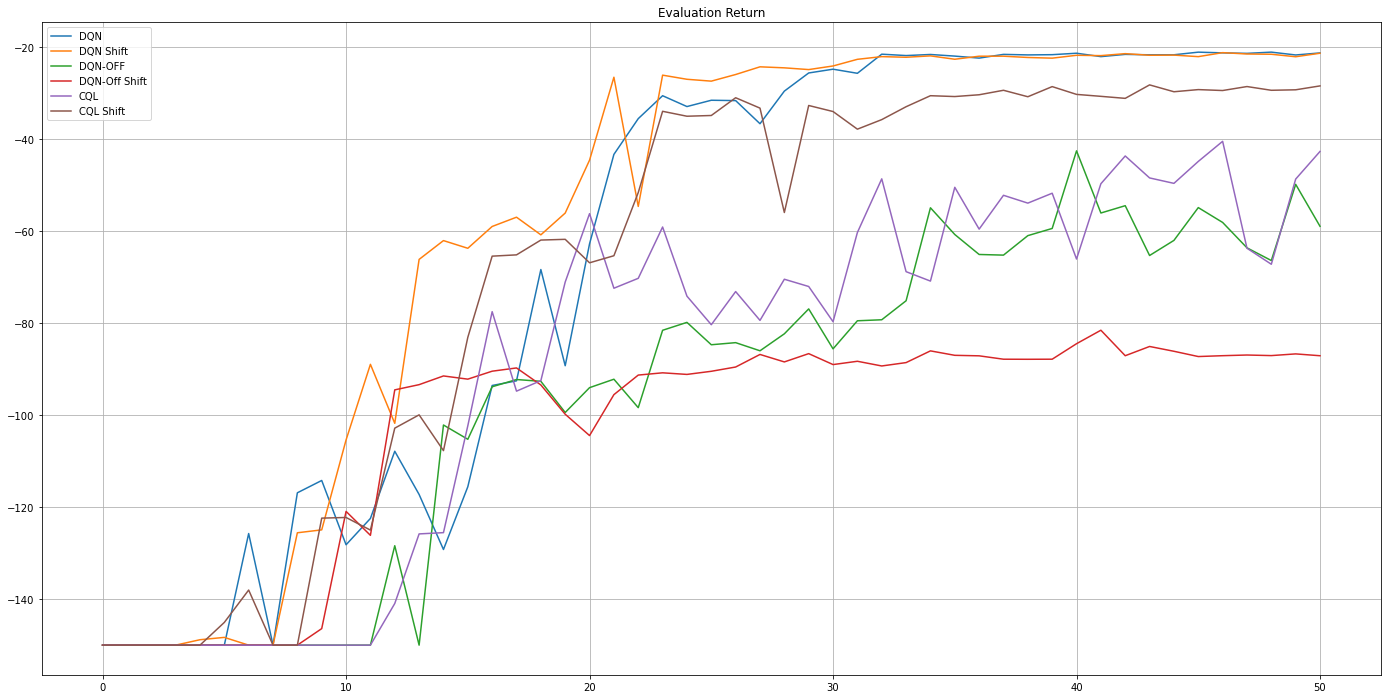
\includegraphics[scale=0.30]{p2/q2-p1-medium-eval-all}

    The chart above shows evaluation return for DQN, Offline DQN and CQL both with bare and transformed (labelled as Shift) rewards.

    \subsubsection{Bare Rewards}

    \hspace*{-0.4in}
    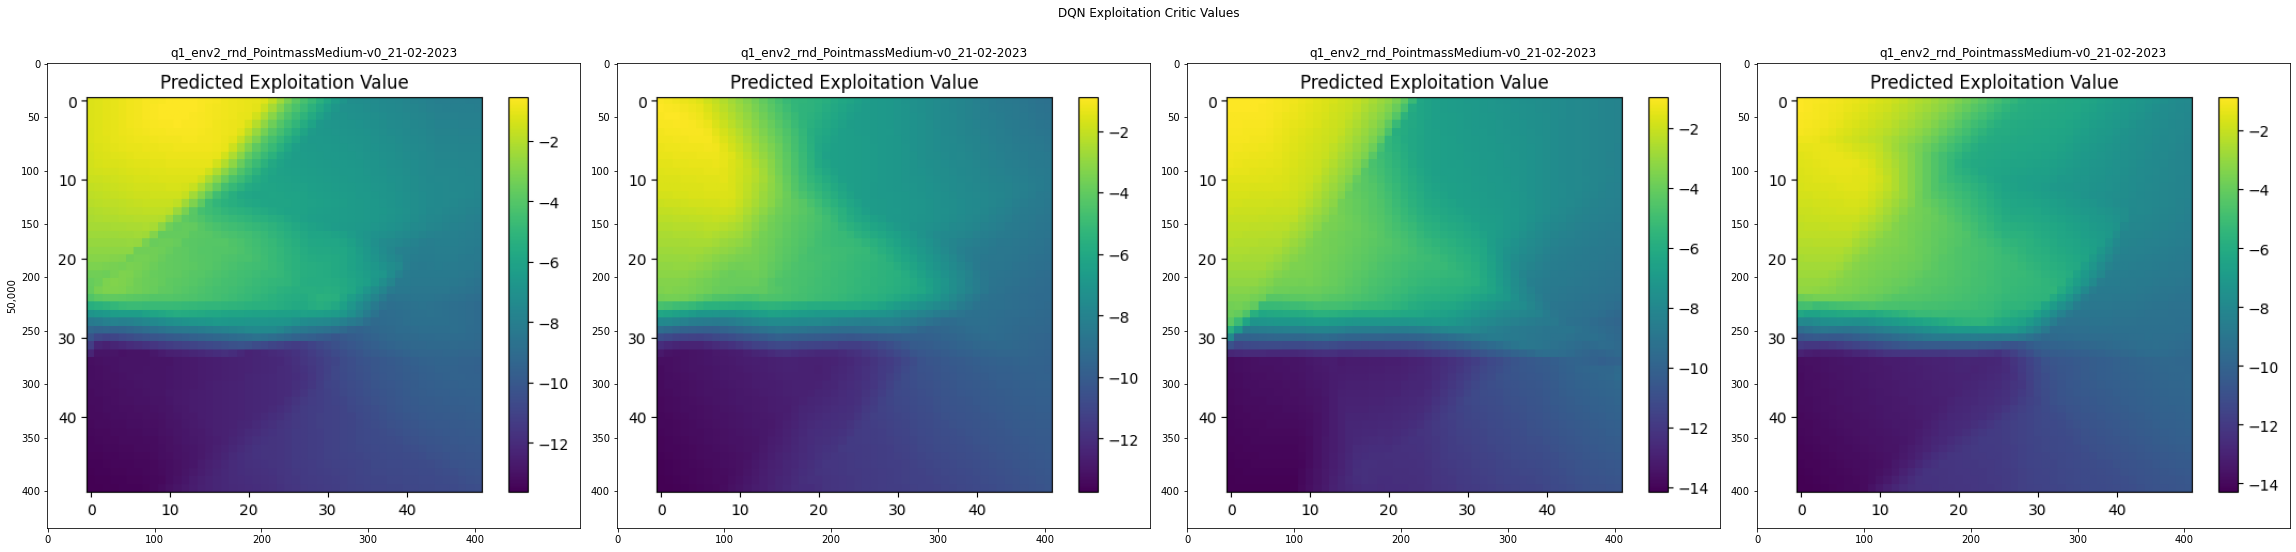
\includegraphics[scale=0.20]{p2/q2-p1-explt-dqn}

    \hspace*{-0.6in}
    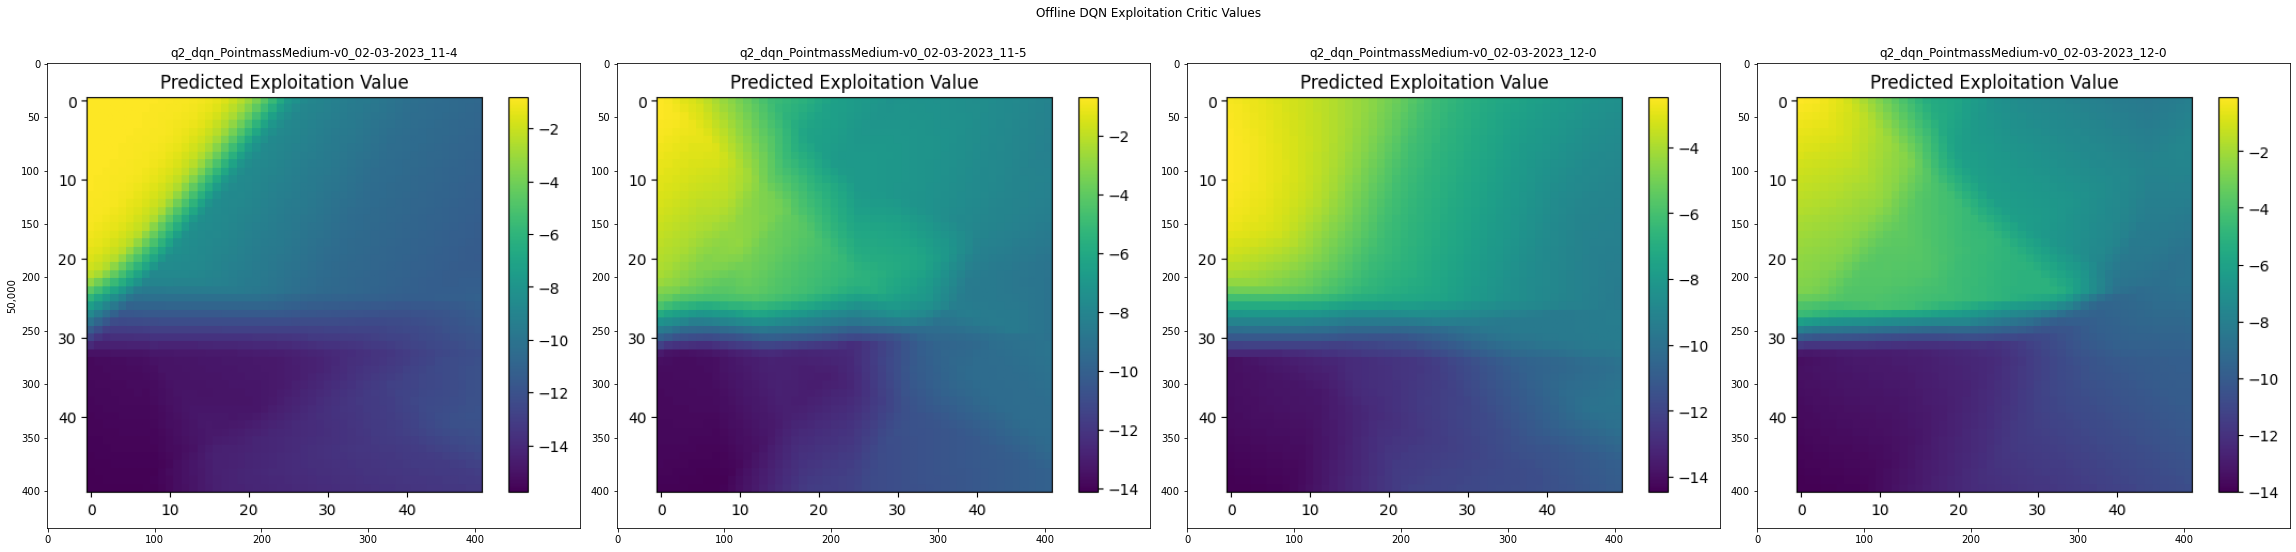
\includegraphics[scale=0.20]{p2/q2-p1-explt-off-dqn}

    \hspace*{-0.6in}
    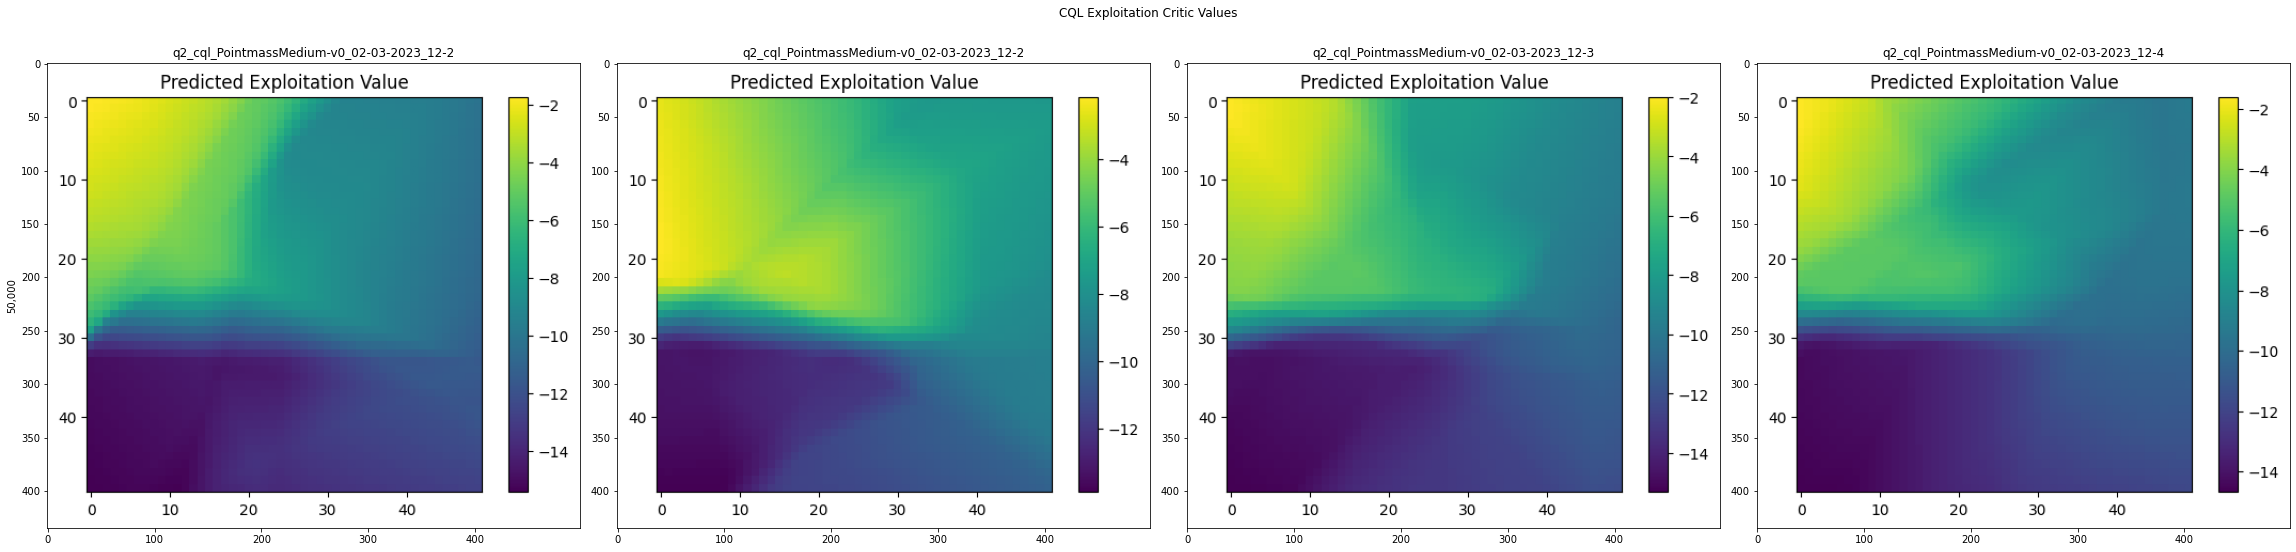
\includegraphics[scale=0.20]{p2/q2-p1-explt-cql}

    Online DQN is the best performer which is expected.

    Offline DQN and CQL performs similarly.
    Their performance is not as good because of the offline settings.

    Does CQL give rise to Q-values that underestimate the Q-values learned via a standard DQN?
    No.
    In the exploration phase, agents rarely reaches the target thus the buffer contains few rewards.
    Few rewards rarely occurs in the samples.
    Additionally, rewards are discounted which makes the effect of already rare rewards less significant.

    \subsubsection{Transformed Rewards}

    As suggested in the homework document rewards are shifted by 1 and scaled by 100.
    This way effects of sparsity and discounting is mitigated.

    Transforming the rewards improves results for online DQN and CQL.

    \hspace*{-0.6in}
    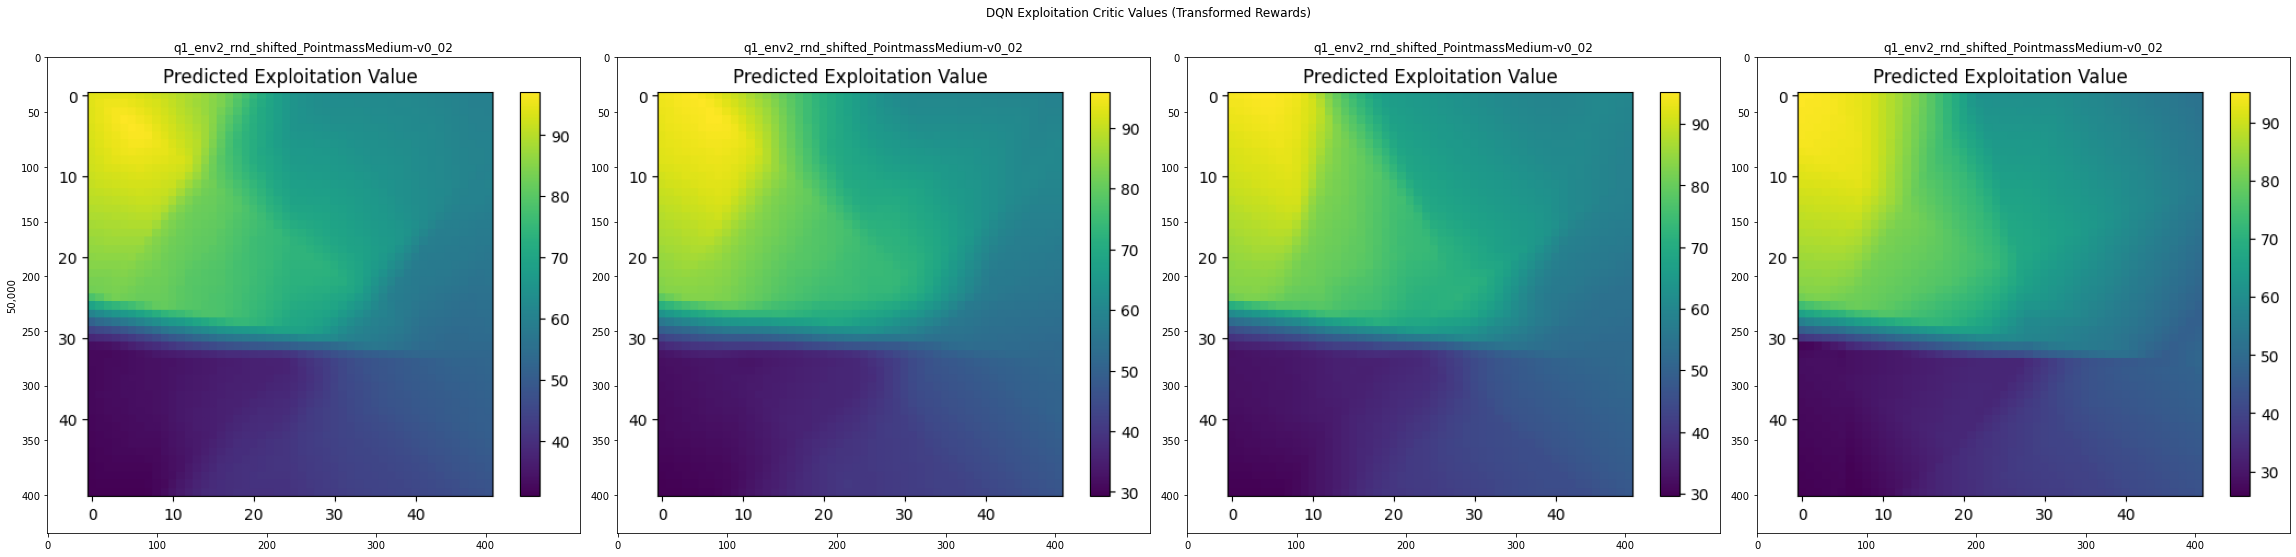
\includegraphics[scale=0.20]{p2/q2-p1-explt-dqn-trans}

    \hspace*{-0.6in}
    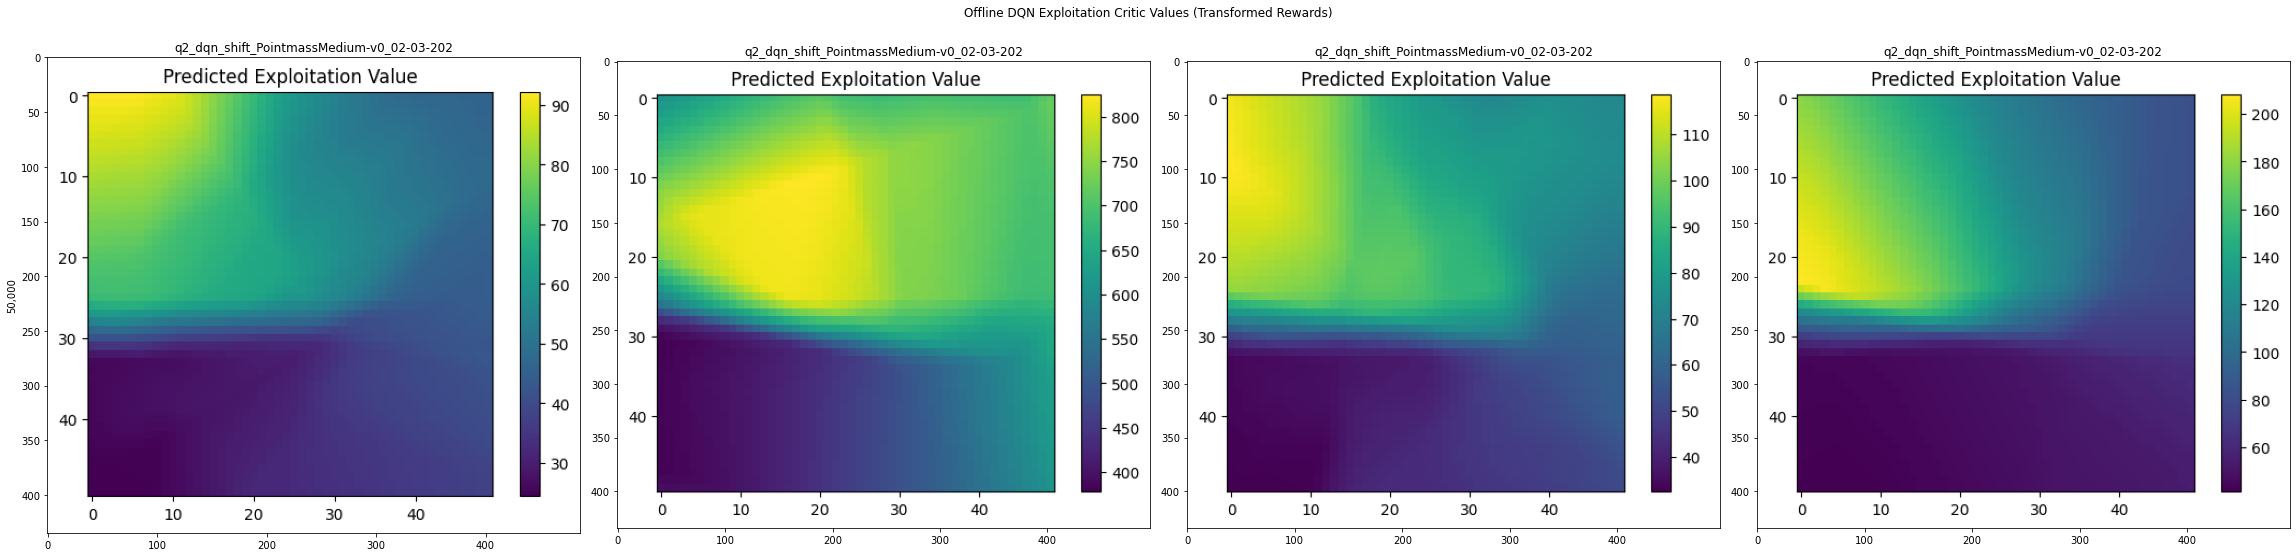
\includegraphics[scale=0.20]{p2/q2-p1-explt-off-dqn-trans}

    \hspace*{-0.6in}
    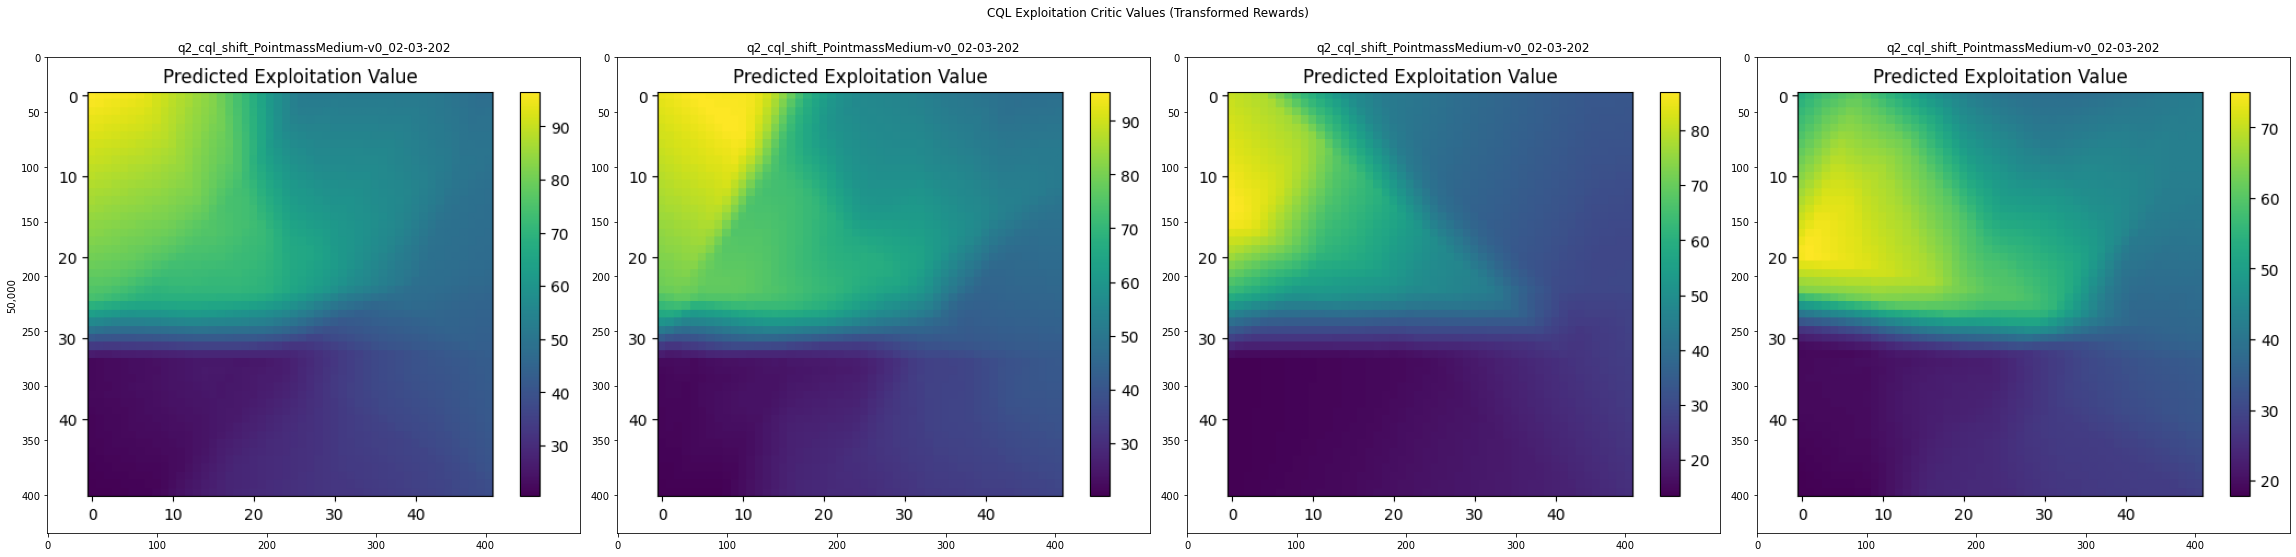
\includegraphics[scale=0.20]{p2/q2-p1-explt-cql-trans}

    With the new results it is easier to derive a conclusion.

    Offline DQN has a tendency to overestimate Q values.
    Offline DQN with transformed rewards performs the worst.

    CQL, on the other hand, has a tendency to underestimate Q values.
    With the transformed rewards, CQL performance improves, almost to the level of online DQN.


    \subsection{Ablation Study}

    An ablation study on the performance of the offline algorithm as a function of the amount of exploration data is performed.
    Transformed rewards are used.

    \hspace*{-0.6in}
    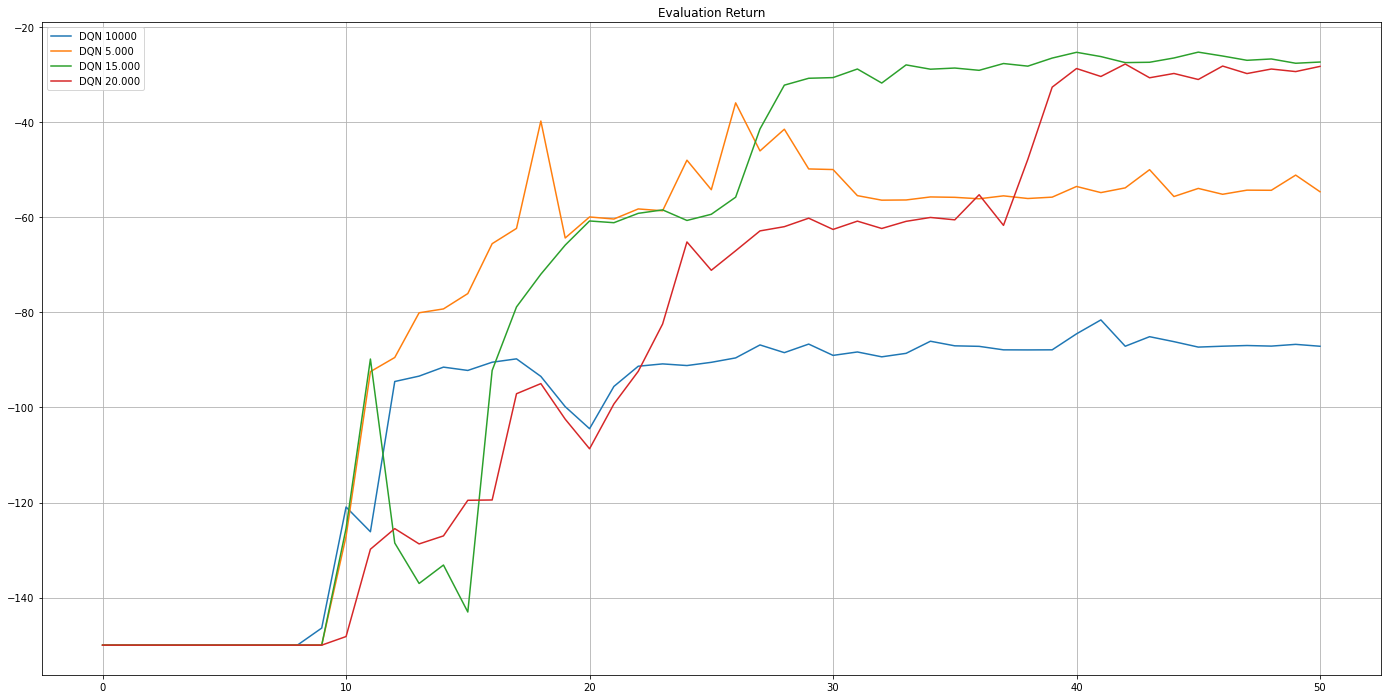
\includegraphics[scale=0.30]{p2-p2/dqn-eval}

    DQN is affected by the number of exploration steps.
    5000 and 10.000 exploration steps perform worse while 15.000 and 20.000 exploration steps perform better.

    \hspace*{-0.6in}
    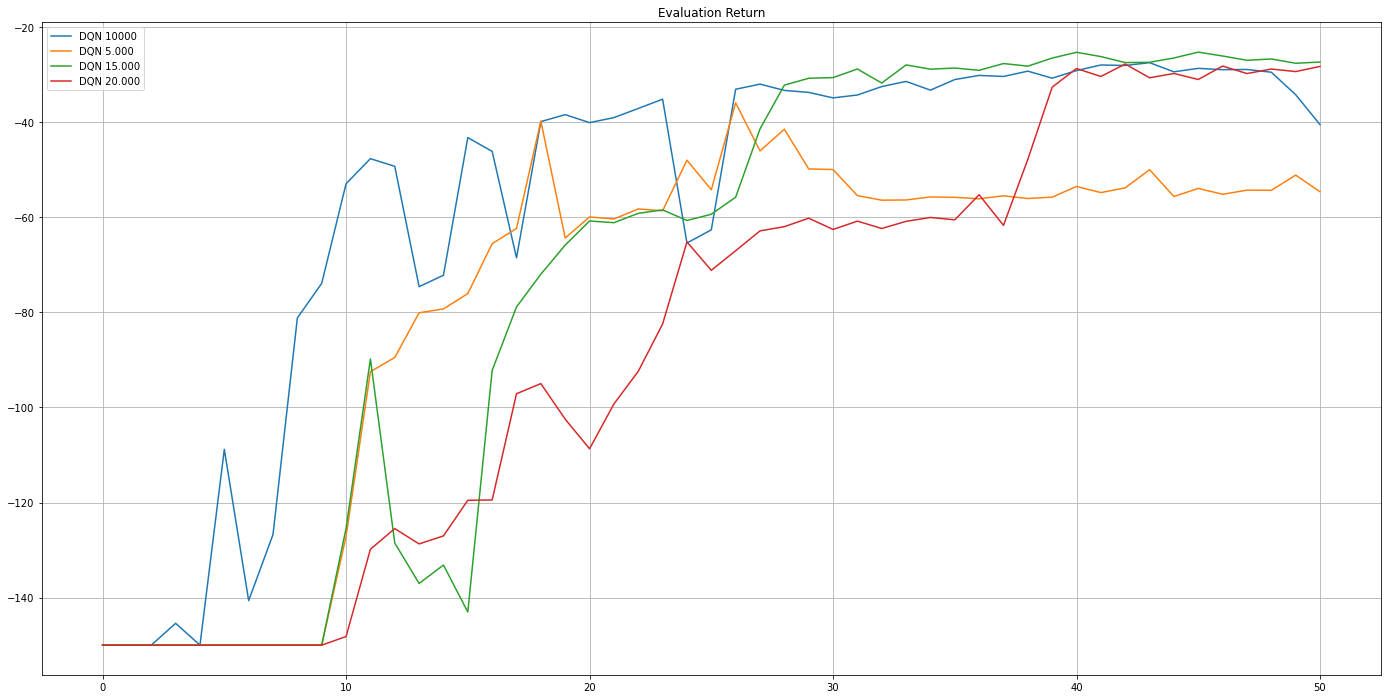
\includegraphics[scale=0.30]{p2-p2/cql-eval}

    CQL performance is not effected by the number of exploration steps, as much.

    \subsection{Alpha Sweep}

    CQL with high or medium alpha values are expected to be better.
    CQL with minimal alpha is expected to perform worse because it gets closer to DQN.

    \hspace*{-0.6in}
    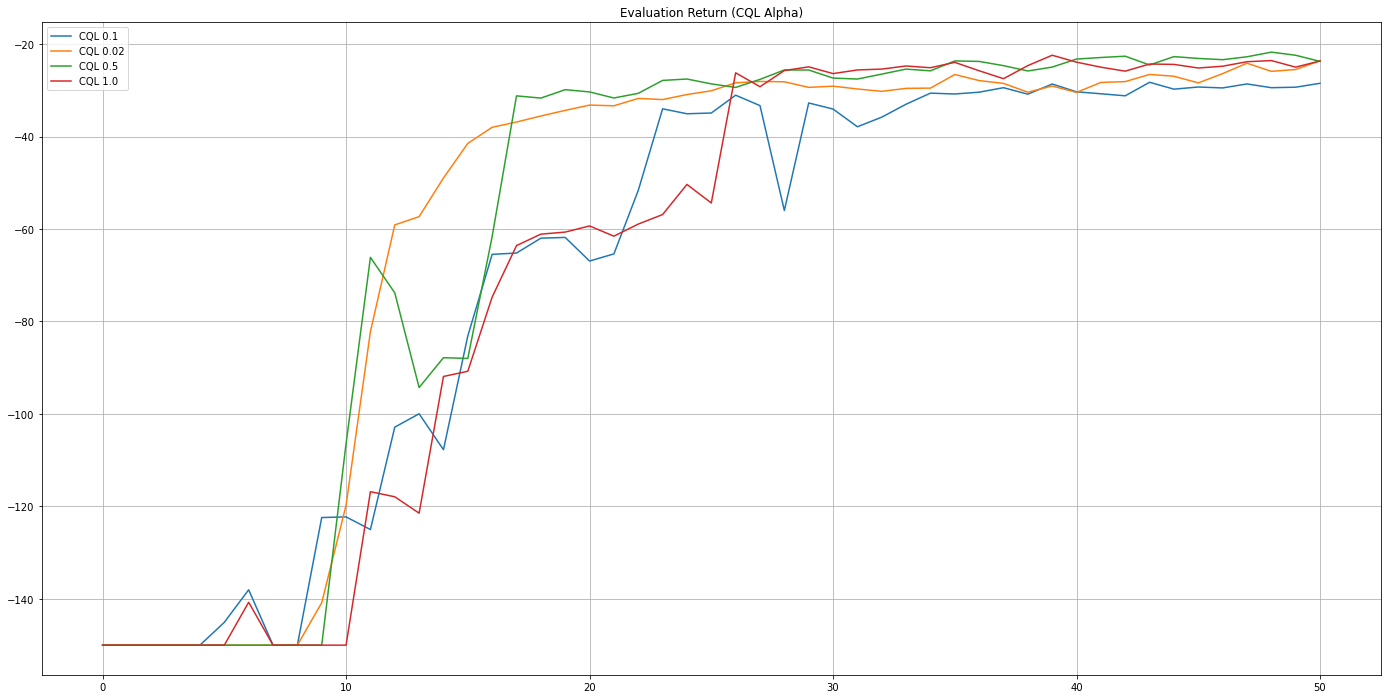
\includegraphics[scale=0.30]{p2-p3/medium}

    In the medium environment there is no significant difference.

    \hspace*{-0.6in}
    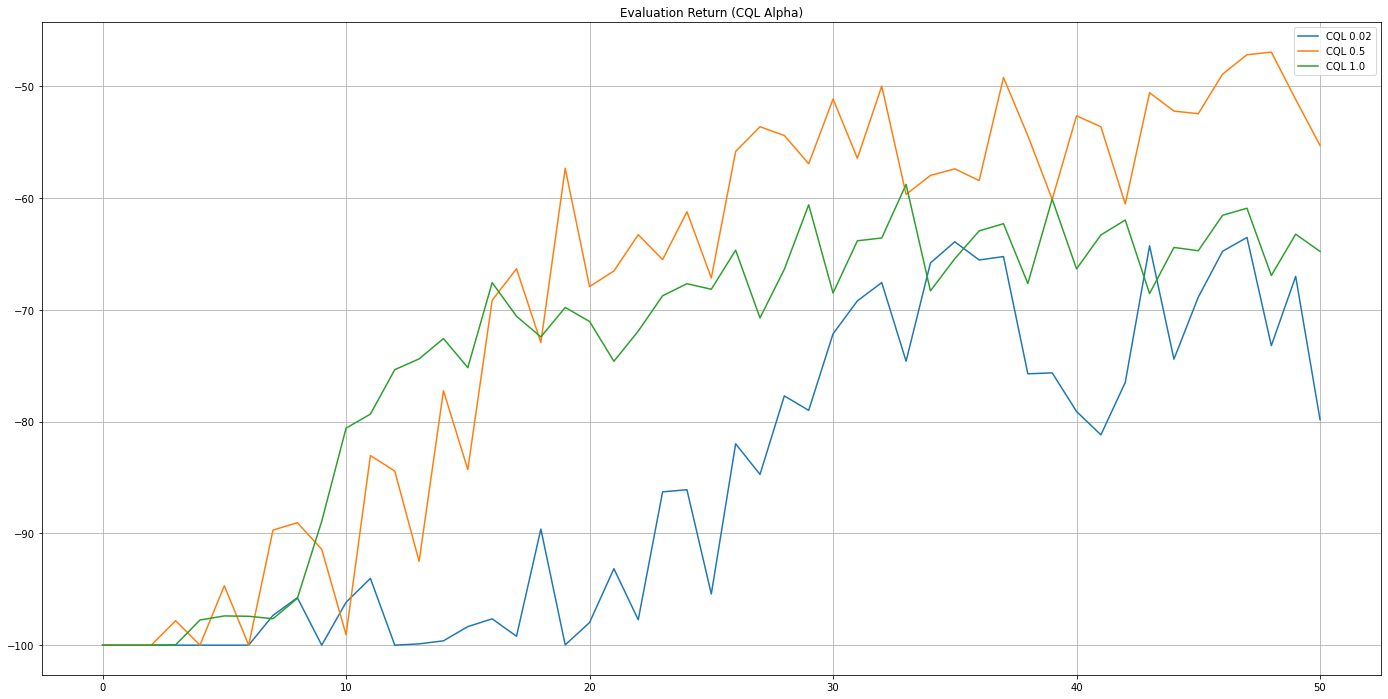
\includegraphics[scale=0.30]{p2-p3/hard}

    In the hard environment the difference is more obvious.

    A medium value of 0.5 performs the best among the selected alpha values.
    A low value of 0.02 performs the worst.


    \section{Part 3: “Supervised” exploration with mixed reward bonuses}

    This question is divided into two parts.
    The first part addresses the original question.
    The second part is an offline extension to the first part.

    A reward transformation of scale = 100 and shift = 1 is used.


    \subsection{“Supervised” exploration with mixed reward bonuses (Online)}

    This section examines the performance of CQL under supervised exploration strategy.
    In supervised exploration, environment reward and exploration reward are augmented to form a mixed reward.

    \subsubsection{Hard Environment}

    \hspace*{-0.3in}
    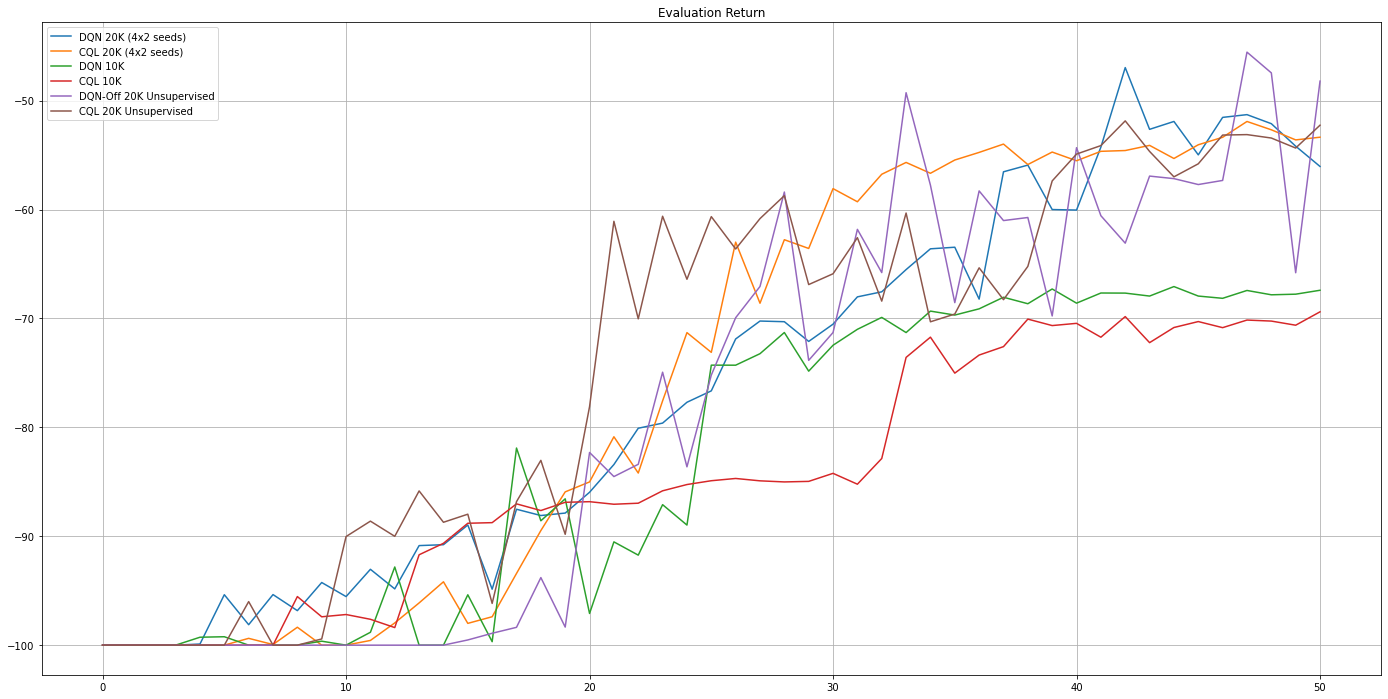
\includegraphics[scale=0.30]{q3-online/hard-eval}

    DQN and CQL compared under 3 different settings.
    In the first setting, 10K exploration steps is used.
    Results are obtained by averaging 4 runs with 4 different seeds.
    In the second setting, 20K exploration steps is used.
    Results are obtained by averaging 8 runs belonging to 4 different seeds.
    In the third setting, which is subpart 2 of part 2, offline training with unsupervised exploration is done for 20K steps.

    Performance of 20K exploration steps is better than 10K exploration case.
    DQN and CQL seems to be performing similar under the same settings.

    Benefit of supervised exploration is not visible.
    CQL with 20K exploration bonuses performs slightly better both in online supervised and offline unsupervised settings.
    Is this an indication of a problem with mixed rewards implementation?
    It is not clear.

    \subsubsection{Medium Environment}

    \hspace*{-0.3in}
    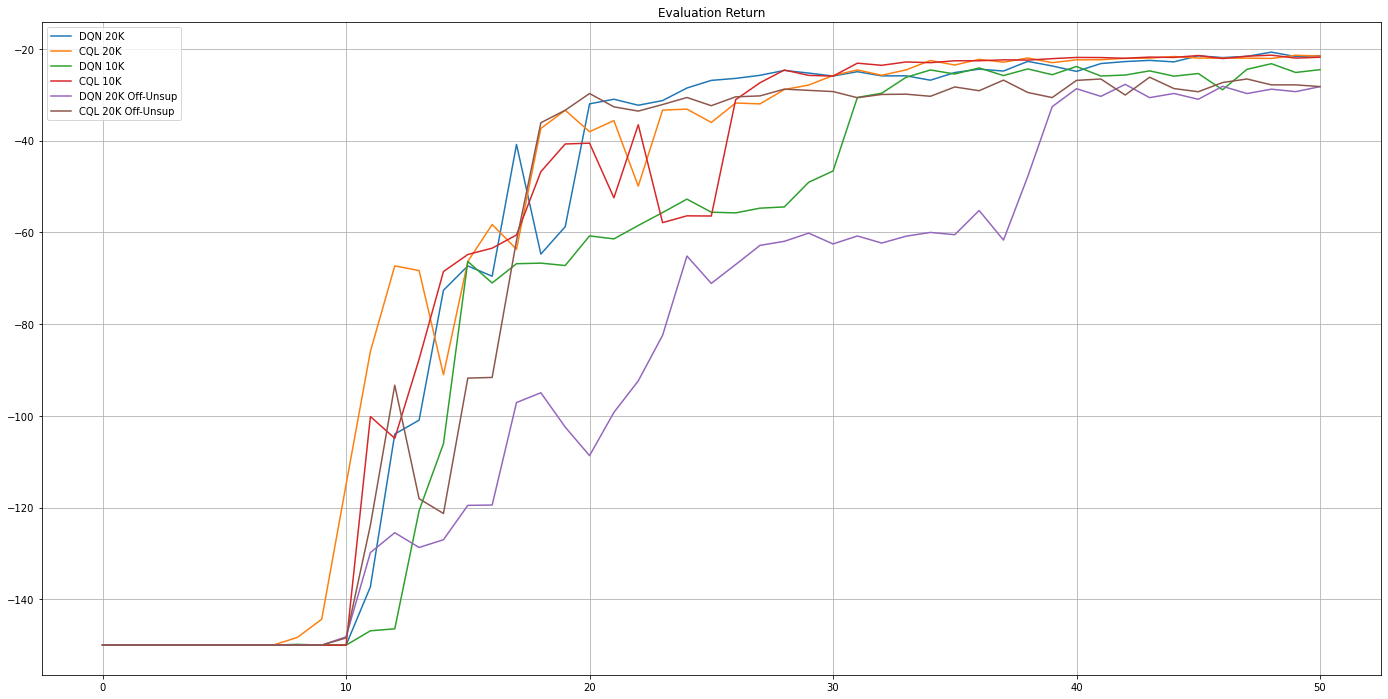
\includegraphics[scale=0.30]{q3-online/medium-eval}

    The setting is the same with the hard environment case.
    Only the environment is different.

    Offline DQN with 20K unsupervised exploration performs worse for some time.
    Being offline it is expected.
    Other settings performs similarly with no obvious difference.

    Where is the benefit of supervised exploration?
    It is not seen.

    \subsection{“Supervised” exploration with mixed reward bonuses (Offline)}

    CQL is an offline algorithm.
    It is more meaningful to compare CQL and DQN under offline settings.

    \subsubsection{Hard Environment}

    \hspace*{-0.3in}
    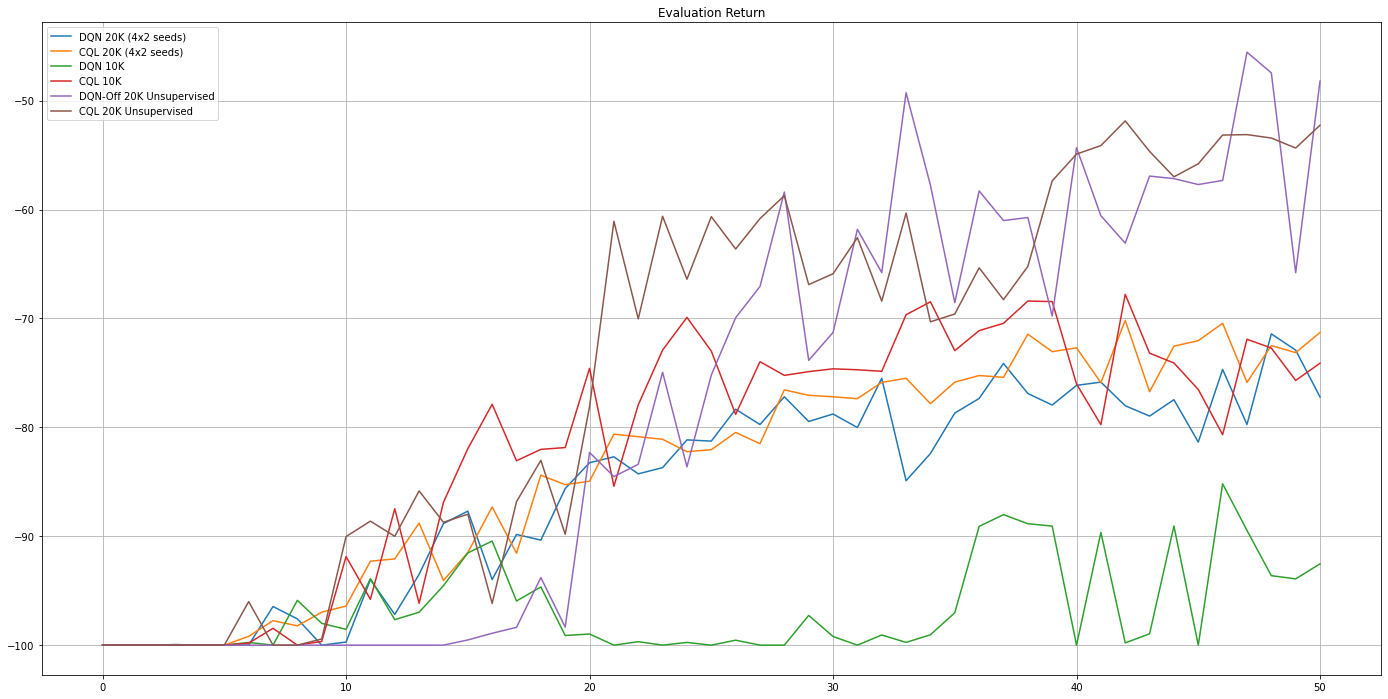
\includegraphics[scale=0.30]{q3-offline/hard-eval}

    Unsupervised offline strategy seems to be better in CQL and DQN case which is not expected.
    Does supervised exploration make things worse?

    \subsubsection{Medium Environment}

    \hspace*{-0.3in}
    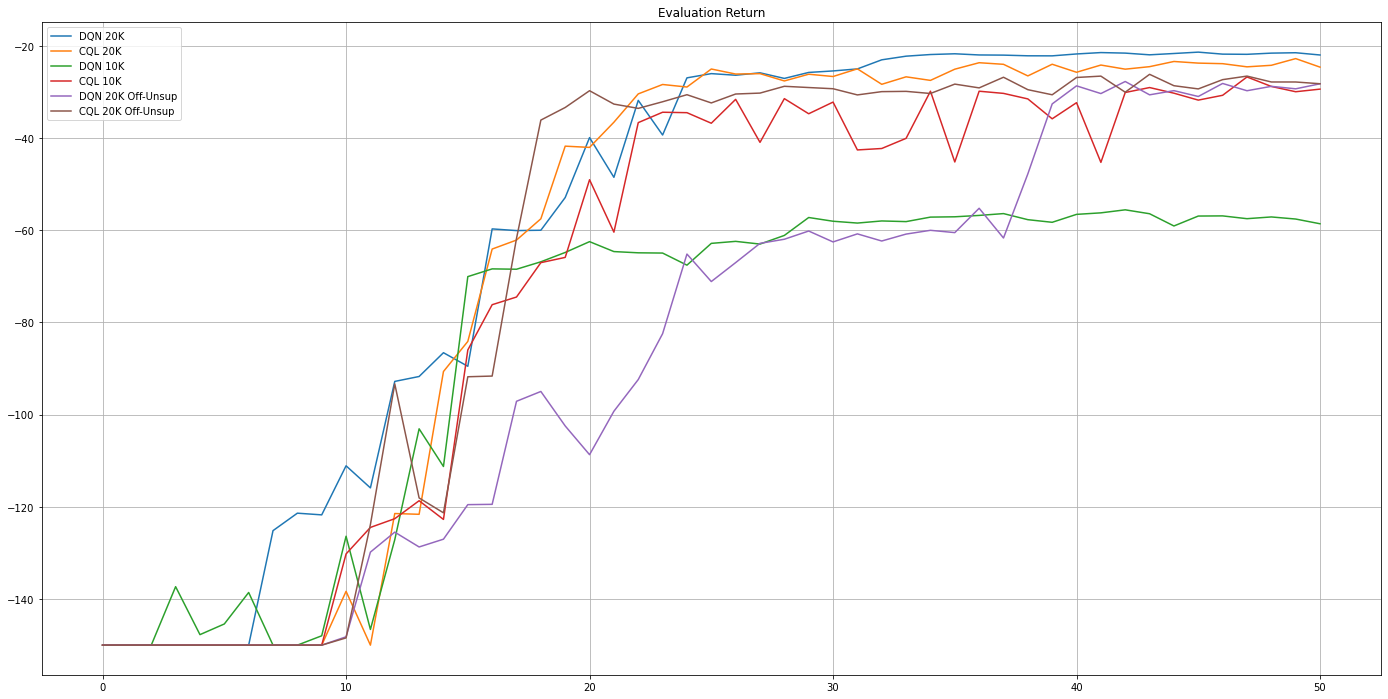
\includegraphics[scale=0.30]{q3-offline/medium-eval}

    There is not significant difference conclude.
    But again supervised exploration shows no improvement.

\end{document}